\documentclass{article}
\usepackage{leonine,amsmath,amssymb,amsthm,graphicx}
\setkeys{Gin}{width=\linewidth,totalheight=\textheight,keepaspectratio}
\graphicspath{{graphics/}}
% Prints a trailing space in a smart way.
\usepackage{xspace}
% Inserts a blank page
\newcommand{\blankpage}{\newpage\hbox{}\thispagestyle{empty}\newpage}
% \usepackage{units}
% Typesets the font size, leading, and measure in the form of 10/12x26 pc.
\newcommand{\measure}[3]{#1/#2$\times$\unit[#3]{pc}}

\theoremstyle{definition}
\newtheorem{pred}[thm]{Prediction}

\title{Cerebellum: Positive Pathway} \author{Eric Purdy}

\begin{document}

\maketitle

\section{Overview}

We posit that the cerebellum as a whole tries to predict the output of
the cerebrum, and takes over the performance of activities that are
sufficiently predictable. Ito \cite{ito} posits a similar theory. The
positive pathway is responsible for producing the outputs of the
cerebellum, some of which will subsequently be filtered out by the
negative pathway (the cortical network whose output is given by the
Purkinje cells).

One of the cerebral outputs that is predicted by the cerebellum is the
input that the cerebrum sends to the cerebellum. One function of the
positive pathway is thus to predict its own input at the next time
step.

As the cerebellum does its work to predict the output of the cerebrum,
it relies on three kinds of information: commands from the cerebrum;
context from the proprioceptive system; and its own internal model of
the state of the cerebrum, the state of the body, and the stte of the
world.

We will refer to sequences of cerebellar outputs as actions, and the
individual cerebellar outputs as elementary actions.

\begin{figure}
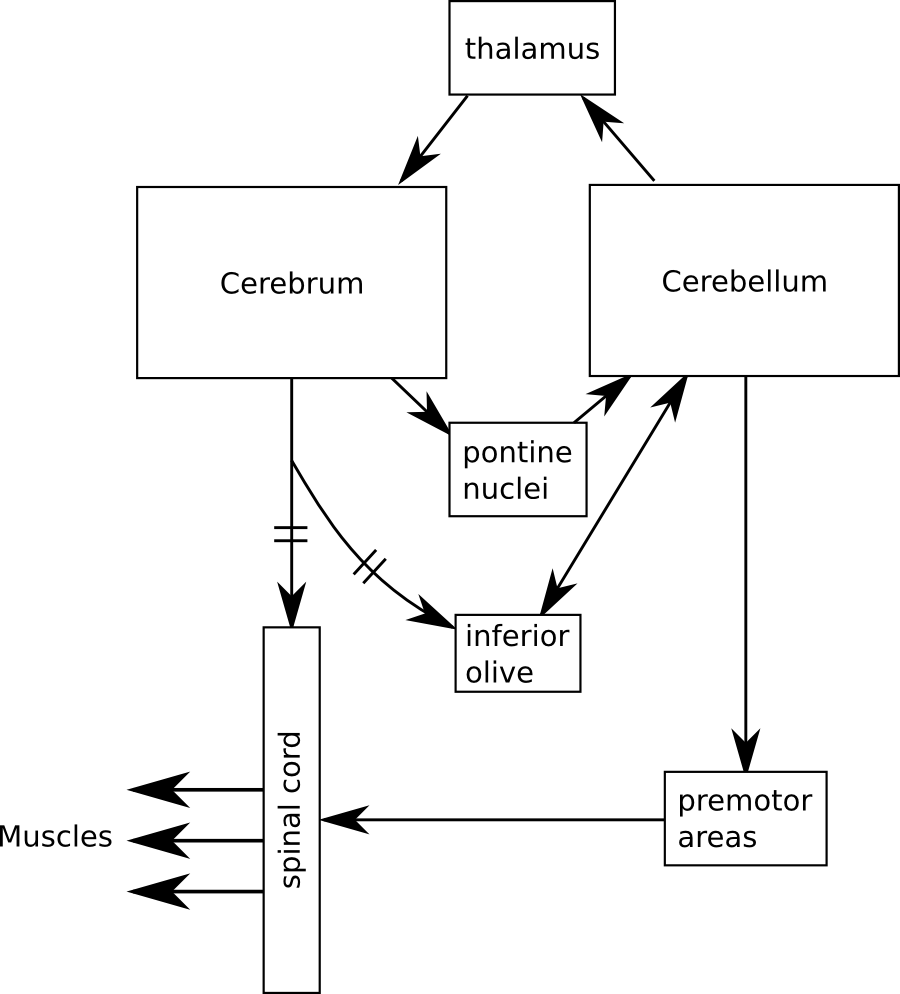
\includegraphics[width=\linewidth]{organization.png}
\caption{Inputs and outputs of the cerebellum. The two arrows marked
  with double lines represent two neural pathways that convey copies
  of the same information.}
\label{fig-organization}
\end{figure}

\subsection{Interface with the Cerebrum}

The cerebrum is able to perform actions by sending commands to the
cerebellum. It is also able to perform actions directly, by issuing
commands to other premotor areas, but a copy of these commands
(``efference copy'') is received by the inferior olive, which relays
the information to the cerebellum. 

It is also worth noting that the inferior olive receives other
information as well, including pain signals. It is probably that the
output of the cerebellum is used as commands in some cases, and as
perceptions in other cases. It is also the case that some perceptions
are immediately mapped to commands that would be appropriate given the
perceptions; the most well-studied example is the nictating membrane
response, which protects the eye from a painful stimulus. The relevant
training signal conveyed by the inferior olive in that case is the
pain signal from the eye, while the relevant output is a closing of
the membrane.

The meaning of each command changes continuously as the parameters and
connections in the cerebellum change. The cerebrum must therefore
continuously relearn what each command does.

One important change is that two commands which are consistently
issued together, one immediately after the other, will eventually be
merged into a single command by the cerebellum. When this happens, the
cerebrum will then learn that issuing the second command is no longer
necessary, and that the meaning of the first command has changed to
include both commands.

Another important change is that, if a command to the cerebellum is
consistently issued at the same time as a non-cerebellar command, the
cerebellum will learn this and add the non-cerebellar command to the
cerebellar command. The cerebrum can then send a single command to the
cerebellum to accomplish what previously took two commands. The
cerebrum will have to learn this fact.

It is also worth noting that random or preexisting connections in the
cerebellum can be used by the cerebrum. We posit that the cerebrum
sometimes tries random cerebellar commands in order to see if they
will be useful for the task at hand. So, if the cerebrum identifies a
set of commands that is useful, it will continue to use it, and the
cerebellum will subsequently modify the meaning of the commands to be
even better suited to the purposes of the cerebrum.

We can formalize this last idea more precisely using the notion of
``epsilon-greedyiness''. Consider that we have a number of possible
actions to take, but we do not know the precise results of each action
(this setting is called the ``multi-armed bandit'' in the probability
and machine learning literature). The epsilon-greedy approach to the
problem is to select, with probability $(1-\epsilon)$, the action that
has so far given the best results. However, with probability
$\epsilon$, we instead choose an action completely at random,
uniformly over the space of available actions. The parameter
$\epsilon$ is generally small, so that we usually take the action that
has worked best in the past. There is a tradeoff between
``exploitation'' (using the action that is currently known to be best)
and ``exploration'' (finding out the effects of new actions, since
they may be better than the currently known best action); the lower
$\epsilon$ is, the more we favor exploitation over exploration.

It is also possible to vary $\epsilon$. One popular approach is to
start with $\epsilon$ fairly large, and then gradually decrease it. As
we gain more experience of the results of each action, it makes sense
that we can spend less time on exploration and more time on
exploitation. There is some evidence that the brain uses such a
strategy. When learning a new action, there is activation in many
parts of the cerebellum (which would be what we expect to see if the
cerebrum is trying random commands). Once the action has become
familiar, the activation of the cerebellum lessens and is concentrated
in smaller regions of the cerebellum.

\subsection{Kinds of cells}

The positive pathway makes use of several kinds of neurons: deep
nuclear cells, and the cells of the inferior olive. It also makes use
of mossy fibers, which are the axons of neurons that can be inside or
outside the cerebellum.

\begin{figure}
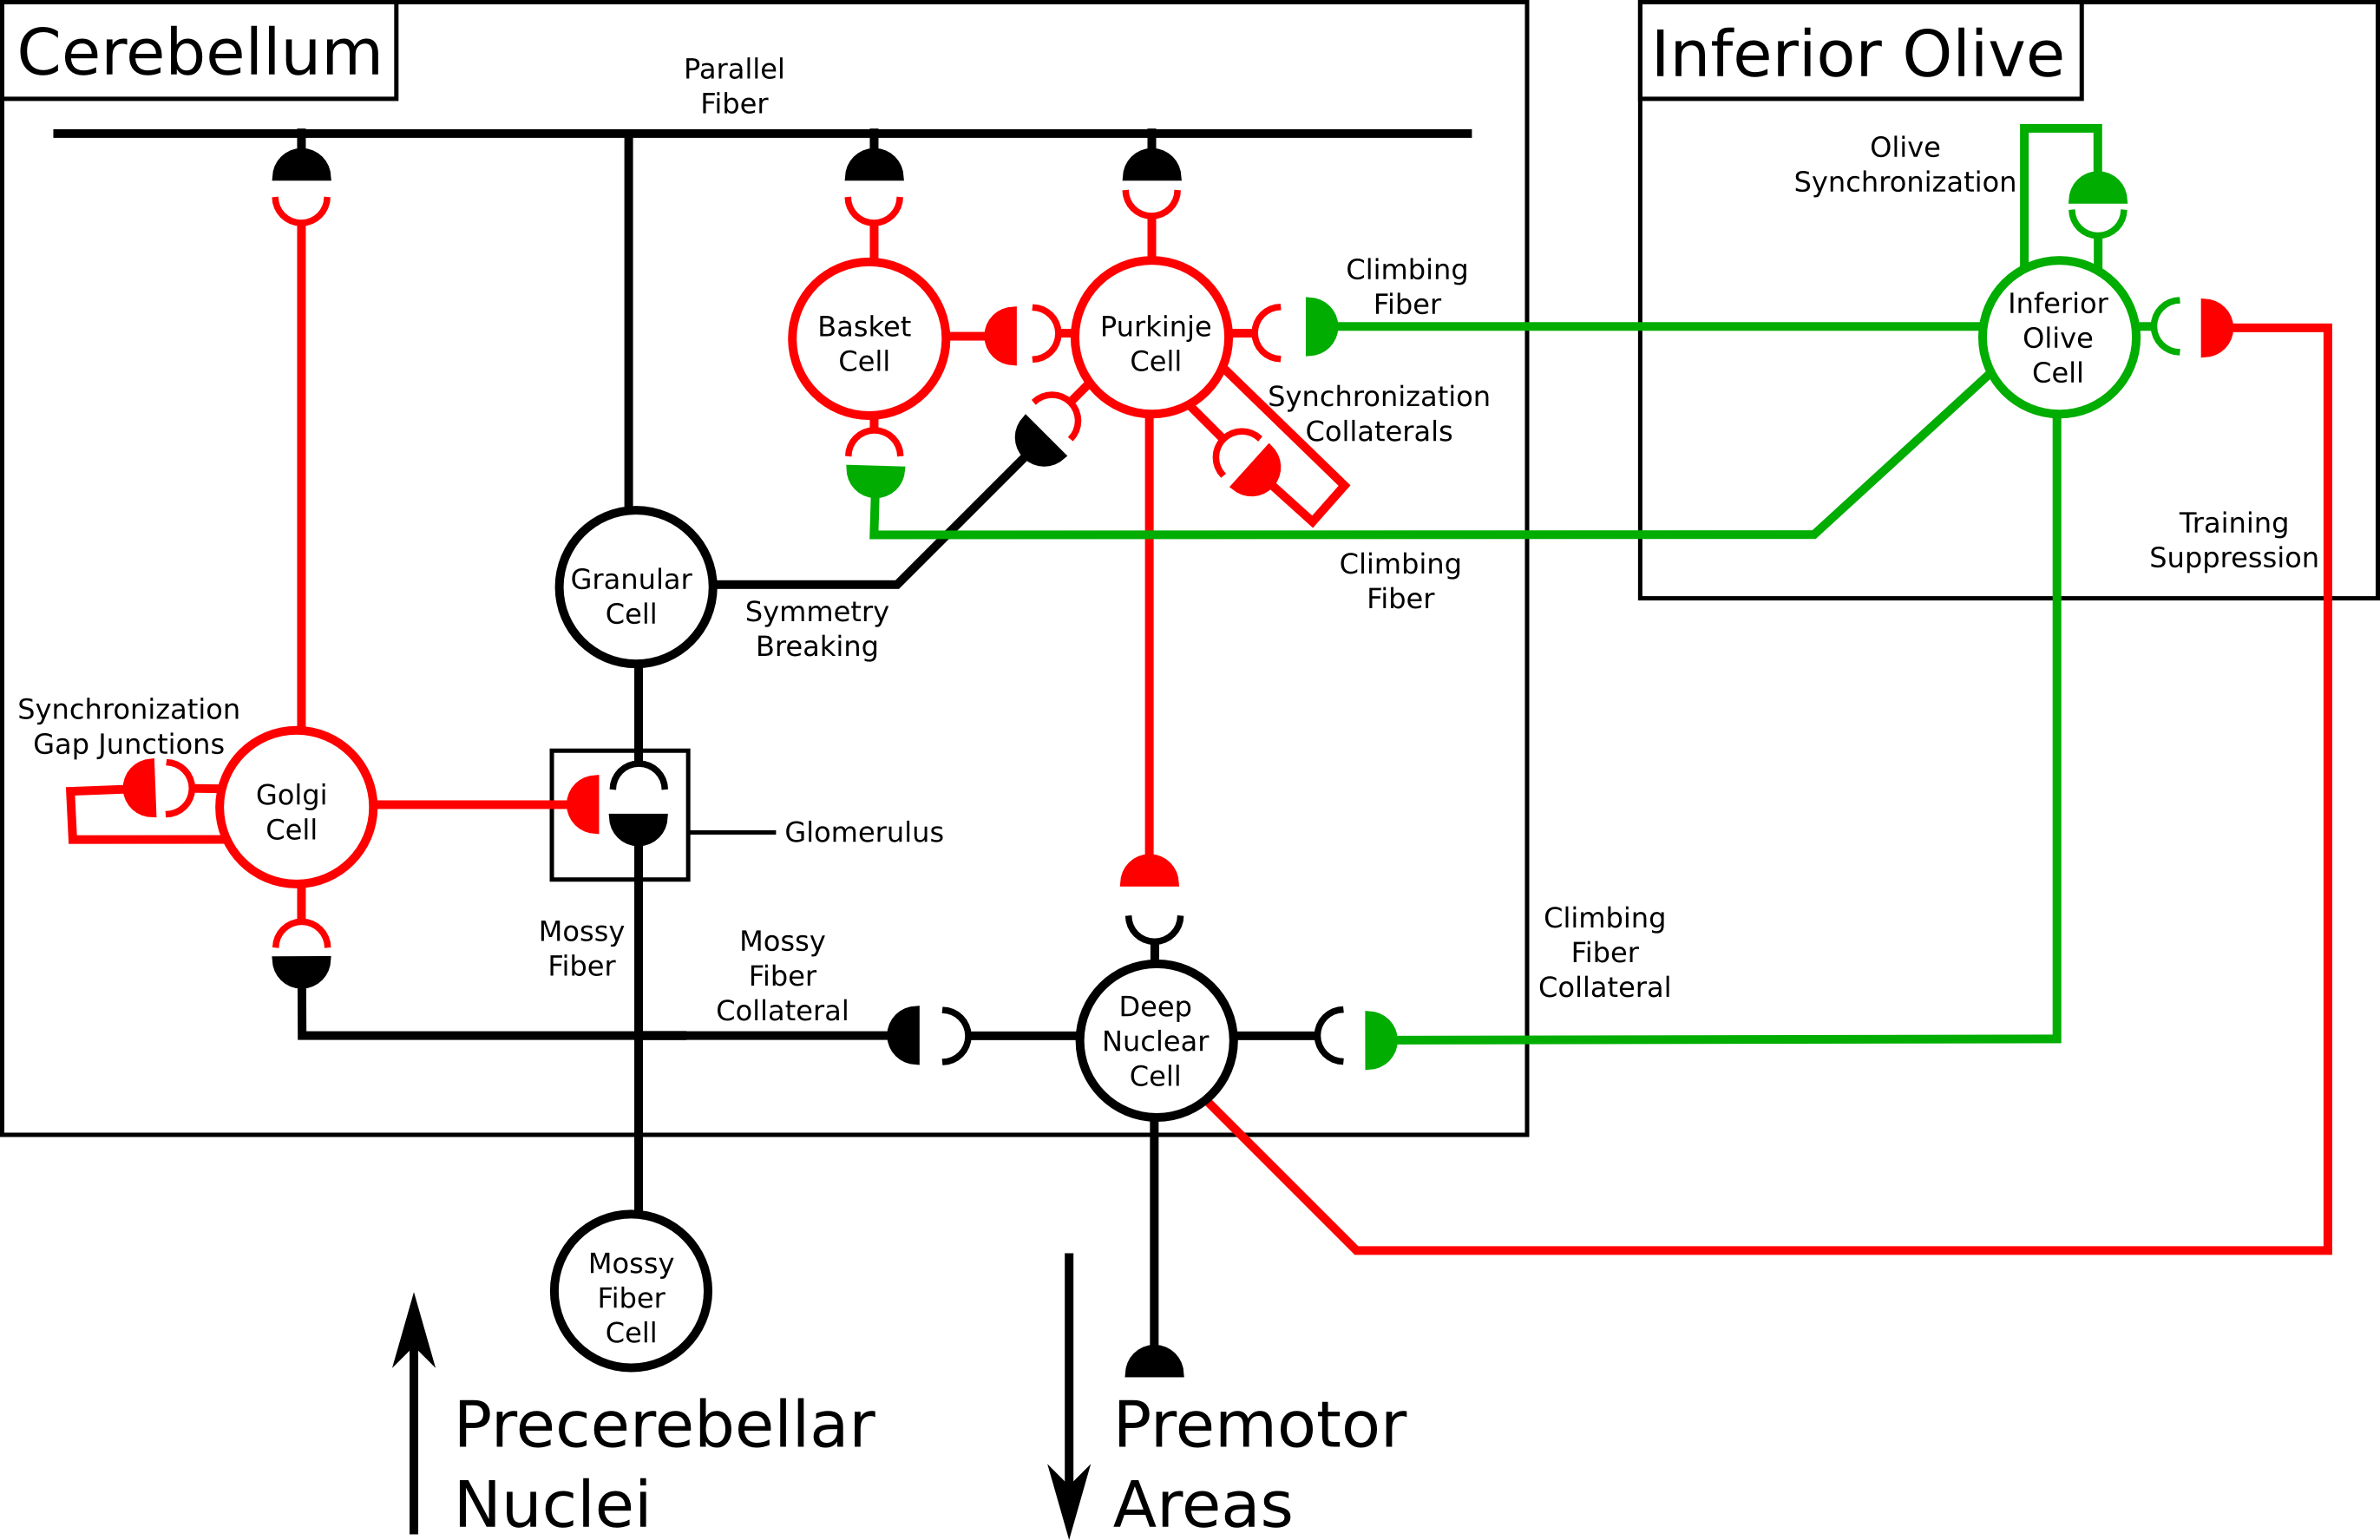
\includegraphics[width=\linewidth]{cells.png}
\caption{Cells of the cerebellum. Excitatory cells are shown in black,
  while inhibitory cells are shown in red. Inputs to a cell are shown
  as an empty half circle, while outputs are shown as a full half
  circle.  Cells of the inferior olive are shown in green, to
  emphasize that their output is used to train the targeted cells;
  they are excitatory. There are two kinds of deep nuclear cell: one
  excitatory and projecting either back into the cerebellum or to
  premotor areas; and one inhibitory and projecting to the inferior
  olive. Since the cells receive the same input, we have simplified
  the picture by identifying them together. It is also worth noting
  that state cells are actually represented twice here: they are both
  ``mossy fiber cells'' and ``deep nuclear cells''.}
\label{fig-cells}
\end{figure}

\begin{figure}
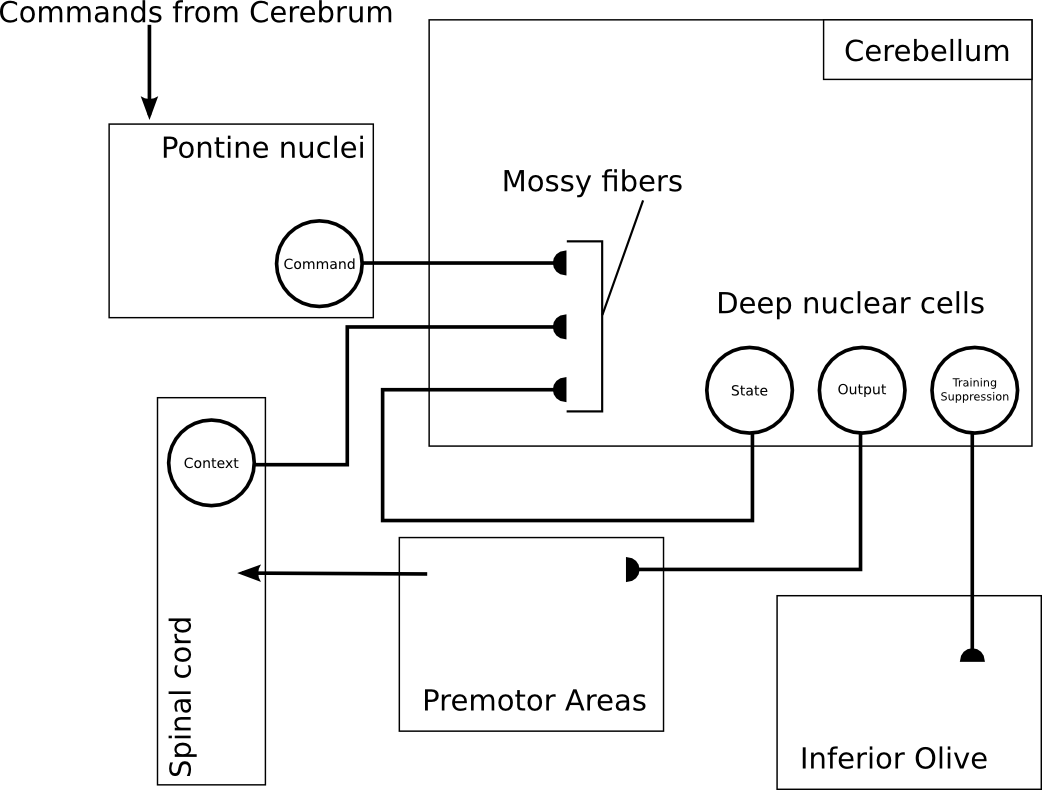
\includegraphics[width=\linewidth]{classification.png}
\caption{Classification of mossy fibers and deep nuclear cells. Note
  that some output cells send their output back to the cerebrum; these
  cells are presumably responsible for cognitive skills, rather than
  motor skills.}
\label{fig-classification}
\end{figure}

All mossy fibers are excitatory. We classify mossy fibers into three
kinds:
\begin{itemize}
\item Command mossy fibers (those coming from
the cerebrum via the pontine nuclei), 
\item Context mossy fibers (those coming from the
spinal cord),  
\item State mossy fibers (those coming from the deep nuclear
cells). 
\end{itemize}
These classes are depicted in Figure \ref{fig-classification}. This
classification is novel, as far as we are aware. These names are meant
to be suggestive, but the true situation is probably more complex, in
that some command cells are probably used mainly to provide context
for other cells' decision making, and some context cells are
interpreted as commands (we call these ``learned reflexes'', and
discuss them in Section \ref{sec-learning-mech}). Nevertheless, we
will use this classification in our discussion.

We classify the deep nuclear cells into three kinds: 
\begin{itemize}
\item State cells (those whose outputs reenter the cerebellum as mossy fibers)
  These cells are excitatory.
\item Output cells (those whose output goes to the spinal cord or back
  to the cerebrum, possibly via intermediate neurons). These cells can
  be either excitatory or inhibitory.
\item Training suppression cells (those whose output goes to the
  inferior olive). These are smaller than the output cells, use GABA
  as a neurotransmitter, and are inhibitory.
\end{itemize}
These classes are again depicted in Figure \ref{fig-classification}.
The classification of state cells vs. output cells is again novel, as
far as we are aware. The difference between these cells and training
suppression cells is already known, although we have not seen the
purpose of training suppression attributed to the training suppression
cells. For simplicity, we assume that each output cell has an
associated training suppression cell which receives the same input, is
active at the same times, and which projects to the same inferior
olive cell that sends a climbing fiber collateral to the given output
cell.

Note that the state cells are deep nuclear cells, and that their axons
are mossy fibers - they receive input as deep nuclear cells and send
output as mossy fibers. We hypothesize that the cerebellum's model of
the state of the cerebrum, the state of the body, and the state of the
world is encoded by firings of the state cells.

\footnote{Word this more formally. What does OK mean? What happens if it's
  not one-to-one? More work, but doesn't invalidate approach. If it's
  just a subset, this has no effect on the mathematical model.} In our
models below, we assume a one-to-one mapping between the command cells
and the state cells. We would also be OK with a one-to-one mapping
between a subset of the command cells and a subset of the state cells,
i.e., the model will still work if some state cells do not receive
input from command cells, or if some command cells do not send input
to state cells. We assume that this mapping is completely arbitrary,
and may be fixed at development. The rest of the system is set up to
learn around this mapping.

Finally, we have the cells of the inferior olive, which are known to
fire when an unexpected movement has occurred. The inferior olive
receives two inputs: an ``efference copy'' of the signals sent from
the cerebrum to the spinal cord, and inhibitory inputs from the deep
nuclear cells that we have termed training suppression cells. A given
inferior olive cell that codes for a particular elementary action thus
fires if the cerebrum produced that movement command, but the
cerebellum did not - thus, it will only fire when that movement occurs
but was not predicted by the cerebellum. This is why it fires on
``unexpected'' movements: expected movements will be produced by the
cerebellum, while unexpected movements will not.

\subsection{State Cells are Implemented as Two or More Cells?}

It is possible that the role played in this document by the state
cells is actually performed by a combination of several cells that
relay information out of and then back into the cerebellum. The theory
would easily adapt to this case if the data suggests it.

\subsection{Competent Performance}

We now give an informal description of the model during performance of
an action. We will give a more formal mathematical model later. The
model is depicted in Figure \ref{fig-positive-overview}.

\footnote{Move figure slightly earlier?}
\begin{figure}
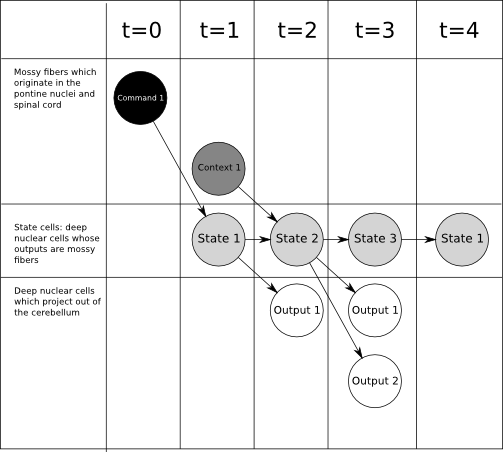
\includegraphics[width=0.95\linewidth]{positive_overview.png}
\caption{Overview of the positive pathway during performance. The
  system receives input through the mossy fibers, which is used to
  maintain a state coded by the activation of a state cell. State
  cells trigger other state cells to fire subsequently. State cells
  also trigger output cells to fire, producing the output of the
  positive pathway as deep nuclear cell firings. Note that the same
  state cell can appear at more than one time step. From $t=2$ to
  $t=3$, we have a timed transition from state cell 2 to state cell
  3. From $t=1$ to $t=2$, we have a waypoint transition, since the
  context cell is used to guide the decision to transition from state
  cell 1 to state cell 2. See text for more discussion of the two
  types of transition.}
\label{fig-positive-overview}
\end{figure}

Consider the act of walking. We need to make a conscious decision to
start walking, but once we start, our body seems to continue the
process on its own. We believe that people with damaged cerebellums
have to plan out such movements every time they execute them.

The cerebrum initiates actions via the command mossy fibers. Each
command cell corresponds to some suite of learned actions. After the
command cell fires, the cerebellum takes over and executes the desired
action.

Every action can be thought of as a series of stages. For instance,
during walking, we push off with one foot, shift our balance slightly
to the other leg, move the foot forward, and then bring it down. In
order to perform the action correctly, the cerebellum has to know what
part of the walking cycle it is in. We hypothesize that such
information is encoded by the state cells, which are the deep nuclear
cells whose outputs are mossy fibers. A state cell is active during a
particular moment in the action.

We assume that there is a one-to-one mapping between output cells and
muscles, so that each output cell produces a single elementary action
when it fires. (This is true only for the regions of the cerebellum
whose outputs go to the spinal cord via premotor areas. Some regions
of the cerebellum send output back to the cerebrum via the thalamus;
we assume that these regions are responsible for cognitive skills. Our
theory applies to these regions as well, but the elementary actions of
those regions do not correspond to muscles.)

A single state cell can control a whole suite of muscles via a number
of different output cells, and those outputs/muscles can overlap with
those of other state cells. During learning, the cerebellum
establishes the relationship between a given state cell and the output
cells is triggers.

Each state cell is responsible for two things, intiating the muscle
contractions appropriate to the moment for which the cell is
responsible (called ``output''), and ensuring that the next state cell
in the sequence fires at the next moment in time (called
``transition''). The information necessary to perform output is
encoded in the synapses between state cells and output cells: the
stronger the synapse, the more likely it is that the state cell will
induce the output cell to fire. This firing will be relayed to the
spinal cord, and will eventually result in a muscle contraction. The
information necessary to perform transition is encoded in the synapses
between the current state cell and other state cells: the stronger the
synapse, the more likely it is that the current state cell will induce
the next state cell to fire at the next moment in time.
\footnote{Strength of synapse can also code intensity of the movement}

Although it is an oversimplification, it is useful to think of only
one state cell being active at a time. The firing of each state cell
then represents how far along we are in executing a given
action. There is then, over short intervals, a one-to-one
correspondence between state cells and time steps in the execution of
an action. Suppose that a given action takes four time steps;
representing it will then require four state cells. The action will be
initiated by a command cell, which will trigger the first state
cell. The first state cell will trigger some number of output cells to
produce muscle contractions, and will also trigger the second state
cell to fire at the next time step. The second state cell will then
trigger a different set of outputs cells, corresponding to the outputs
that are needed at the second time step of the action. The second
state cell will also trigger the third state cell, and so on.

There are two different ways to decide that a transition is needed:
either we know that we want to be in a particular state at the next
moment in time, or some particular information comes in that suggests
that we need to change to a particular state. We call the first way a
``timed transition'', and the second way a ``waypoint transition''. A
timed transition simply encodes the information that one state should
follow another at a particular later time. For instance, during a
blink, the eye should close and then open; the commands to open the
eyelid should start a fixed time after the commands to close the
eyelid. A waypoint transition encodes the information that the state
of the body in the world has changed. For instance, during walking,
once the leg has successfully been raised the appropriate amount, this
information can be relayed back to the cerebellum, and the system can
advance to the next state, corresponding, say, to the point in the
walking process where the leg begins to be brought back down.

The end of a movement can be encoded by simply having no strong
synapses from the last state cell in the chain to any subsequent state
cell. 
\footnote{Alternatively, there can be another command to stop the
motion. Stop commands require a more complex model than the other
phenomena discussed here, so we will defer discussion until later. 

Give a reference to when. Also really need to think about stop
commands.}

The organization of the positive pathway during competent performance
is described in Figure \ref{fig-positive-overview}.

\subsection{Learning mechanisms}
\label{sec-learning-mech}

We now give an informal description of the model during learning. We
will give a more formal mathematical model later. 

\begin{figure}
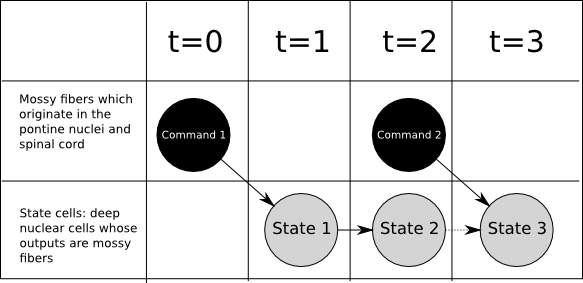
\includegraphics[width=0.95\linewidth]{positive_transition.png}
\caption{Learning of positive pathway transition functions. If command
  1 is consistently followed by command 2 two time steps later, the
  system will learn the transition represented by the dashed arrow.}
\label{fig-positive-transition}
\end{figure}

There are two different kinds of learning that take place in the
positive pathway: learning of transitions, and learning of outputs.

Transition learning allows the cerebellum to merge two skills that it
has already learned. If one command is consistently issued before
another command, and the delay between them is consistently $t$ steps
later, then the cerebellum will learn to transition between
them. After this has taken place, the first command will automatically
cause the same effects as if the second command had followed $t$ steps
later. We can think of this as ``movement chaining'': the movement
coded for by one command cell will be automatically followed by the
movement coded for by a second command cell.

Transition learning takes place at the synapses between two state
cells. If one state cell is consistently active at the time step
directly before another state cell is active, then the synapse between
them will be strengthened. This coincidence can be caused by the
consistent issuance of two commands a fixed distance apart, as shown
in Figure \ref{fig-positive-transition}. There are other ways to cause
the coincidence. For instance, if a particular context cell
consistently fires at the time step before a particular state cell
fires, then a transition will be learned between the context cell and
the state cell - this can be thought of as a ``learned reflex'',
since it will result in the cerebellum automatically initiating an
action in response to some sensory input, without the need for
involvement of the cerebrum.

\begin{figure}
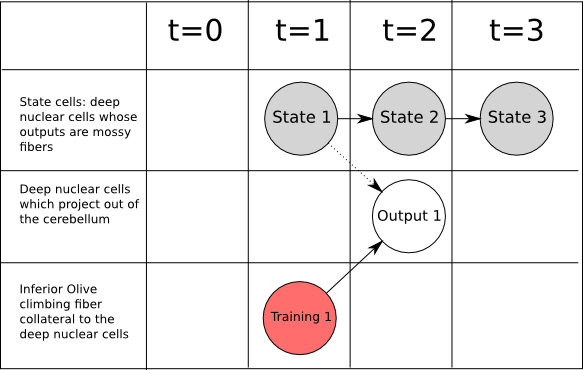
\includegraphics[width=0.95\linewidth]{positive_output.png}
\caption{Learning of positive pathway output functions. If state cell
  1 is consistently active at the same time as training cell 1, the
  system will learn that state cell 1 should trigger output 1, as
  represented by the dashed arrow. Note that learning should actually
  be maximized when the training cell fires slightly after the state
  cell fires (100 msec?) - this is Prediction
  \ref{pred-positive-delay}.}
\label{fig-positive-output}
\end{figure}

Output learning establishes the mapping between states and outputs,
allowing the cerebellum to issue commands to the muscles via the
spinal cord. Each state cell has the ability to trigger several output
cells, which code for particular muscle contractions. The cerebellum
is taught which output cells should be fired at a particular movement
by the firing of the inferior olive. The climbing fiber collateral
causes the firing of the output cell that corresponds to the movement
that the inferior olive cell codes for. Output learning is triggered
when the firing of a particular inferior olive cell consistently
coincides with the firing of a particular state cell, as shown in
Figure \ref{fig-positive-output}.

\section{Negative Pathway as a Training Signal}

We think it is likely that the input from the training cells in the
inferior olive is not the only source of training input for the output
cells. It is also possible that the output cells can be triggered by a
pause in the inhibitory firing of the Purkinje cells in the negative
pathway; this is called ``rebound excitation''. Under this hypothesis,
a pause in the firing of the Purkinje cells that synapse on a given
output cell would be taken as ground truth for the training of the
output cell.

The negative pathway is capable of learning a more complex function
than the positive pathway, so it makes sense for the positive pathway
to learn from it. It seems likely that the negative pathway's storage
is more volatile (does not last as long), and that the parameters and
connections of the positive pathway last longer. This is similar to a
theory proposed by Mauk.

Therefore, while we refer below to training cells as the source of the
training signal for output cells, this should be understood to also
include rebound excitation from pauses in the firing of negative
pathway Purkinje cells.

It is also possible that the positive pathway learns transitions from
the negative pathway. However, for this to be the case, the negative
pathway would have to receive input from the inferior olive that tells
it when a command has been issued. The inferior olive would thus have
to receive a copy of the command signals that are sent to the
cerebellum via the pontine nuclei. In the absence of such a copy being
sent, the negative pathway could not learn when to fire state cells,
and thus would not be a useful signal in learning transitions. If the
necessary connections exist, though, learning transitions from the
negative pathway would make the system far more capable.

\section{Garbage Collection}

If a particular skill is unused for sufficiently long, it would make
sense for the cerebellum to reclaim the resources that are used to
represent it. Thus it would make sense for the synaptic weights to
gradually decay when neither of the neurons is active for a
sufficiently long period of time. We refer to this process as
``garbage collection''. It would return the unused part of the system
to a neutral state in which new actions can be easily learned.

\section{Mathematical models}

First, some notation. We break time into discrete points labeled by
integers. If $k$ is the name of a neuron, then we let $k(t)$ be $1$ if
neuron $k$ fires at time $t$, and $0$ if neuron $k$ does not fire at
time $t$.

We will assume that time is broken up into discrete, regularly spaced
steps, and that all firings occur exactly at the time of a particular
time step. This is obviously not realistic, but it makes everything
simpler to write down and discuss. The model should still work with
the messy firing timing that the brain actually uses.

We give four mathematical models of the positive pathway, largely for
the sake of understanding. Each model is more complex than the model
before it. Except for the third and fourth models, each model is a
special case of the next model. The fourth and last model is the only
one which seems biologically feasible. Even more complex models are
possible, which might perform better; We have stopped at the simplest
model which is biologically feasible and likely to perform reasonably
well.

Although the first three models are phrased in terms of single
neurons, they can also be thought of in a different way. What we refer
to as state cells in those models can be thought of as particular
combinations of actual state cells being active in Model 3. So a
``state'' of the system corresponds to a subset of the state cells
being active, and for each pair of states $S_1, S_2$, there is some
probability that we will transition from the $S_1$ to $S_2$. Trying to
use the learning rules in Models 0, 1, and 2 would not work in this
setting, because there are too many possible states, so we are
unlikely to have enough training data to accurately set all the
probabilities. Fortunately, the learning rule proposed in Model 3 is
able to use a much smaller amount of data, and is biologically
feasible.

\subsection{Model 0: Linearly ordered state cells}

The simplest possible model that is worth discussing is the linearly
ordered model. This model is able to learn a list of elementary
actions to perform in a given order. It is not able to learn a looping
activity, like walking. It is not able to merge two actions into a
single action - it can only grow an action by adding additional
elementary actions at the end of it. (This is a slight
oversimplification; it is possible to merge two actions if they happen
to align correctly, but this is not particularly likely to happen.)
This model is depicted in Figure \ref{fig-model0}.

\begin{figure}
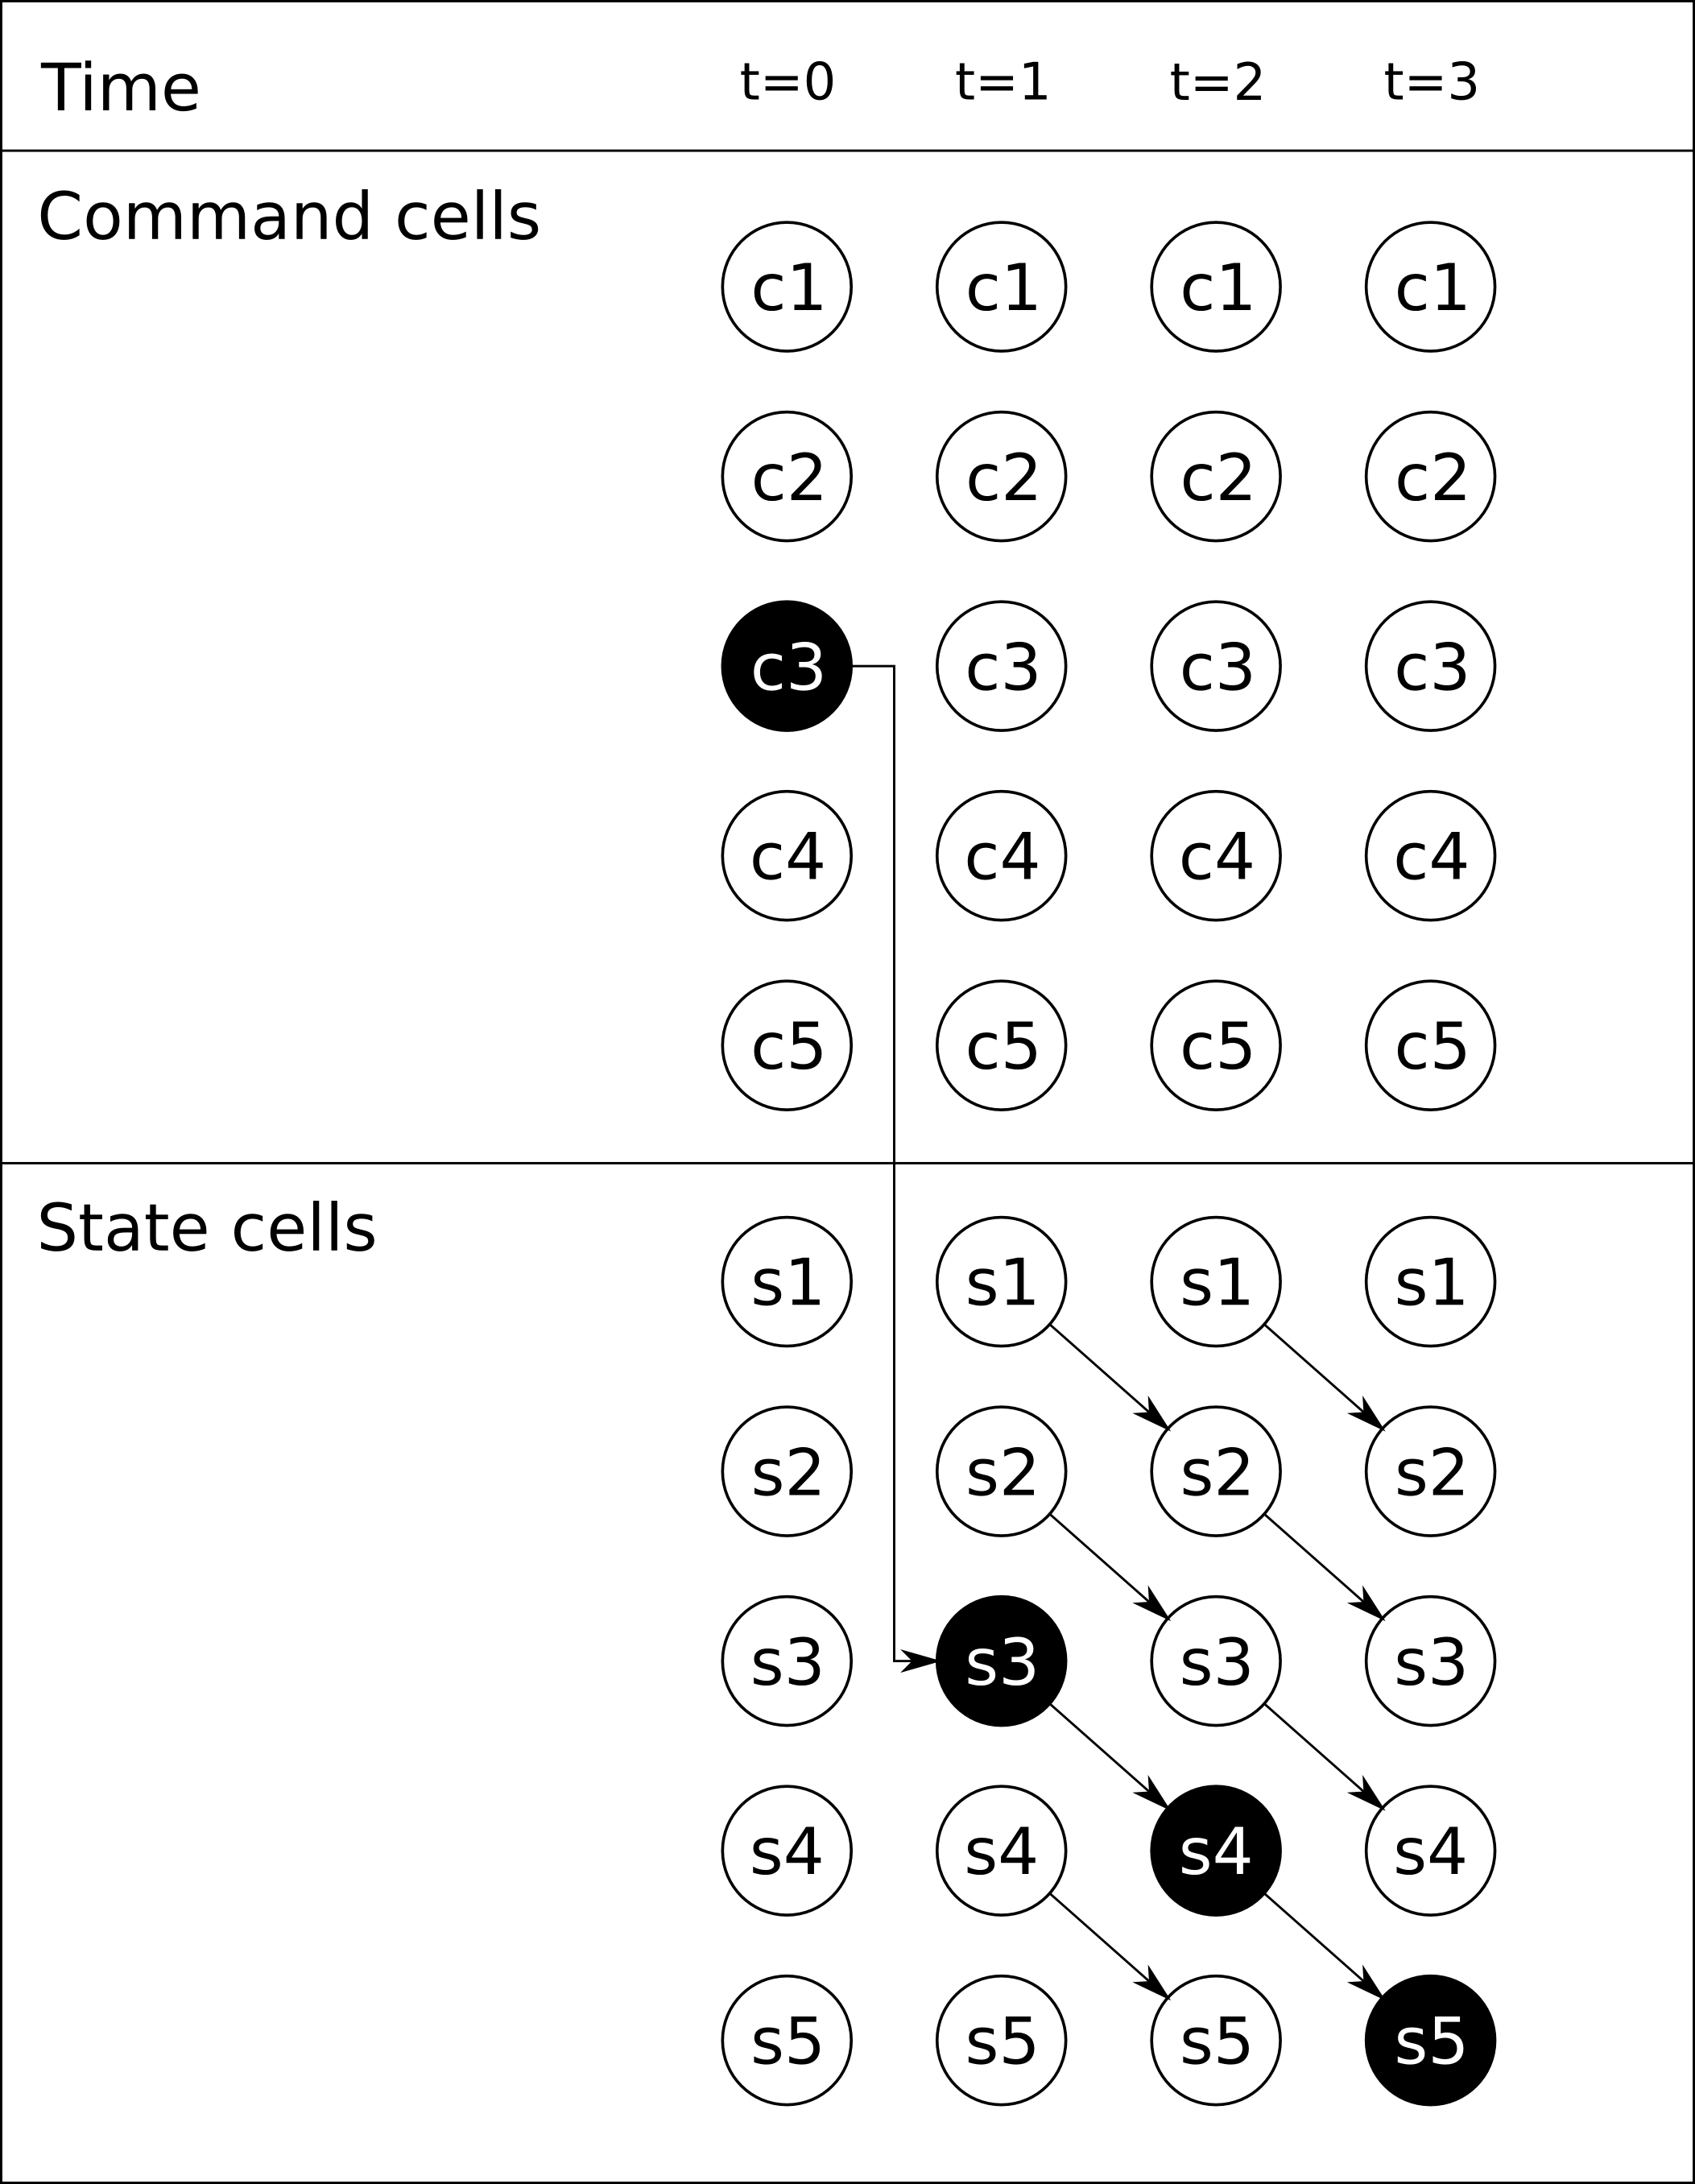
\includegraphics[width=\linewidth]{positive_model0.png}
\caption{Model 0. Each column represents a time step. Each row
  represents a particular neuron. Each circle represents a particular
  neuron at a particular time step; the circle is filled if that
  neuron fires at that time step. Arrows represent synapses between
  neurons, but many of them have been omitted for clarity. Note that
  each command cell $c_i$ excites the corresponding state cell $s_i$,
  and that each state cell $s_i$ excites the next state cell $s_i$.}
\label{fig-model0}
\end{figure}

In this model, the state cells are arranged so that each one receives
input from one state cell and gives output to one other state cell,
and they are arranged in a line. If one state cell fires, the next one
in line probably fires; here ``probably'' means that it fires with a
certain probability, and this probability is a learned parameter. Let
the state cells be denoted by $s_1, \dots, s_n$. If a state cell $s_i$
fires at time $t$, then it is more likely that $s_{i+1}$, the next
state cell in the line, fires at time $t+1$. For the time being, it is
impossible for two state cells to fire at the same time; we will
remove this restriction later.

For this simple model we will assume that the command cells are in
one-to-one correspondence with the state cells. Let the command cells
be denoted by $c_1, \dots, c_n$. We will assume that if the command
cell $c_i$ fires at time $t$, then the state cell $s_i$ is guaranteed
to fire at time $t+1$. If $c_i$ does not fire at time $t$, then it is
still possible for $s_i$ to fire at time $t+1$, but only if state cell
$s_{i-1}$ fires at time $t$. For the time being, it is impossible for
two command cells to fire at the same time.

We have the cells of the inferior olive, which we will denote by $t_1,
\dots, t_m$ (t for training).

Finally, we have the output cells. We will denote the output cells by
$o_1, \dots, o_m$. We do not assume any correspondence between output
cells and state cells, but we do assume that the output cells are in
one-to-one correspondence with the cells of the inferior olive. If
$t_i$ fires at time $t$, then $o_i$ is guaranteed to fire at time
$t+1$. $t_i$ fires when the overall system should produce output
$o_i$, but failed to.

We can express all of the above in the following equations, where
$a(t)=1$ if the neuron $a$ fires at time step $t$, and $a(t)=0$ if it
did not fire at time step $t$.
\begin{align*}
P \left[ s_i(t)=1 | c_i(t-1)=1 \right] &= 1 \\
P \left[ s_i(t)=1 | s_{i-1}(t-1)=0, c_i(t-1)=0 \right] &= 0\\
P \left[ s_i(t)=1 | s_{i-1}(t-1)=1, \forall j, c_j(t-1)=0 \right] &= p_i\\
P \left[ o_j(t)=1 | t_j(t-1)=1 \right] &= 1 \\
P \left[ o_j(t)=1 | t_j(t-1)=0, s_i(t-1)=1 \right] &= q_{ij} \\
P \left[ o_j(t)=1 | t_j(t-1)=0, (\forall i) s_i(t-1)=1 \right] &= 0,
\end{align*}
where the $p_i$ and $q_{ij}$ are parameters that are learned over
time. Recall that only one $s_i$ may be active at any one time in this
model, and that only one $c_i$ can fire at a particular time.

How do we learn $p_i$? Given a set of observations of $s_1, \dots,
s_n$ over time, it is simply the observed conditional probability that
$s_{i-1}$ fired immediately before $s_i$, conditioned on the firing of
$s_{i-1}$.
$$p_i = \frac{\mbox{\# $t$ such that $s_i(t)=1, s_{i-1}(t-1)=1$}}
{\mbox{\# $t$ such that $s_{i-1}(t-1)=1$}}.$$

How do we learn $q_{ij}$? Given a set of observations of $s_1, \dots,
s_n$ and $o_1, \dots, o_m$ over time, it is simply the observed
conditional probability that $s_i$ fired immediately before $o_j$,
conditioned on the firing of $s_i$.
$$q_{ij} = \frac{\mbox{\# $t$ such that $o_j(t)=1, s_i(t-1)=1$}}
{\mbox{\# $t$ such that $s_i(t-1)=1$}}.$$

It is common to set the parameters of a probabilistic model to
maximize the likelihood of some observed data.  Note that neither of
the above rules is the maximum likelihood setting of parameters, since
we don't look at whether a firing of $s_i$ was caused by $s_{i-1}$
firing or by $c_i$ firing, and we don't look at whether a firing of
$o_j$ was caused by $s_i$ or by $t_j$ firing. This is important,
because it allows the system to change its parameters in response to
the sequence of commands observed, and to the training signals from
the inferior olive. 

We can think of these rules as a kind of maximum likelihood
algorithm. Rather than setting parameters to maximize the likelihood
of the outputs given the inputs, we maximize the probability that the
cerebellum would have produced those outputs {\em without the given
  inputs}.

This model is not biologically feasible because there is no mechanism
to ensure that only one state cell is active at a given time.

\subsection{Model 1: Hidden Markov Model}

\begin{figure}
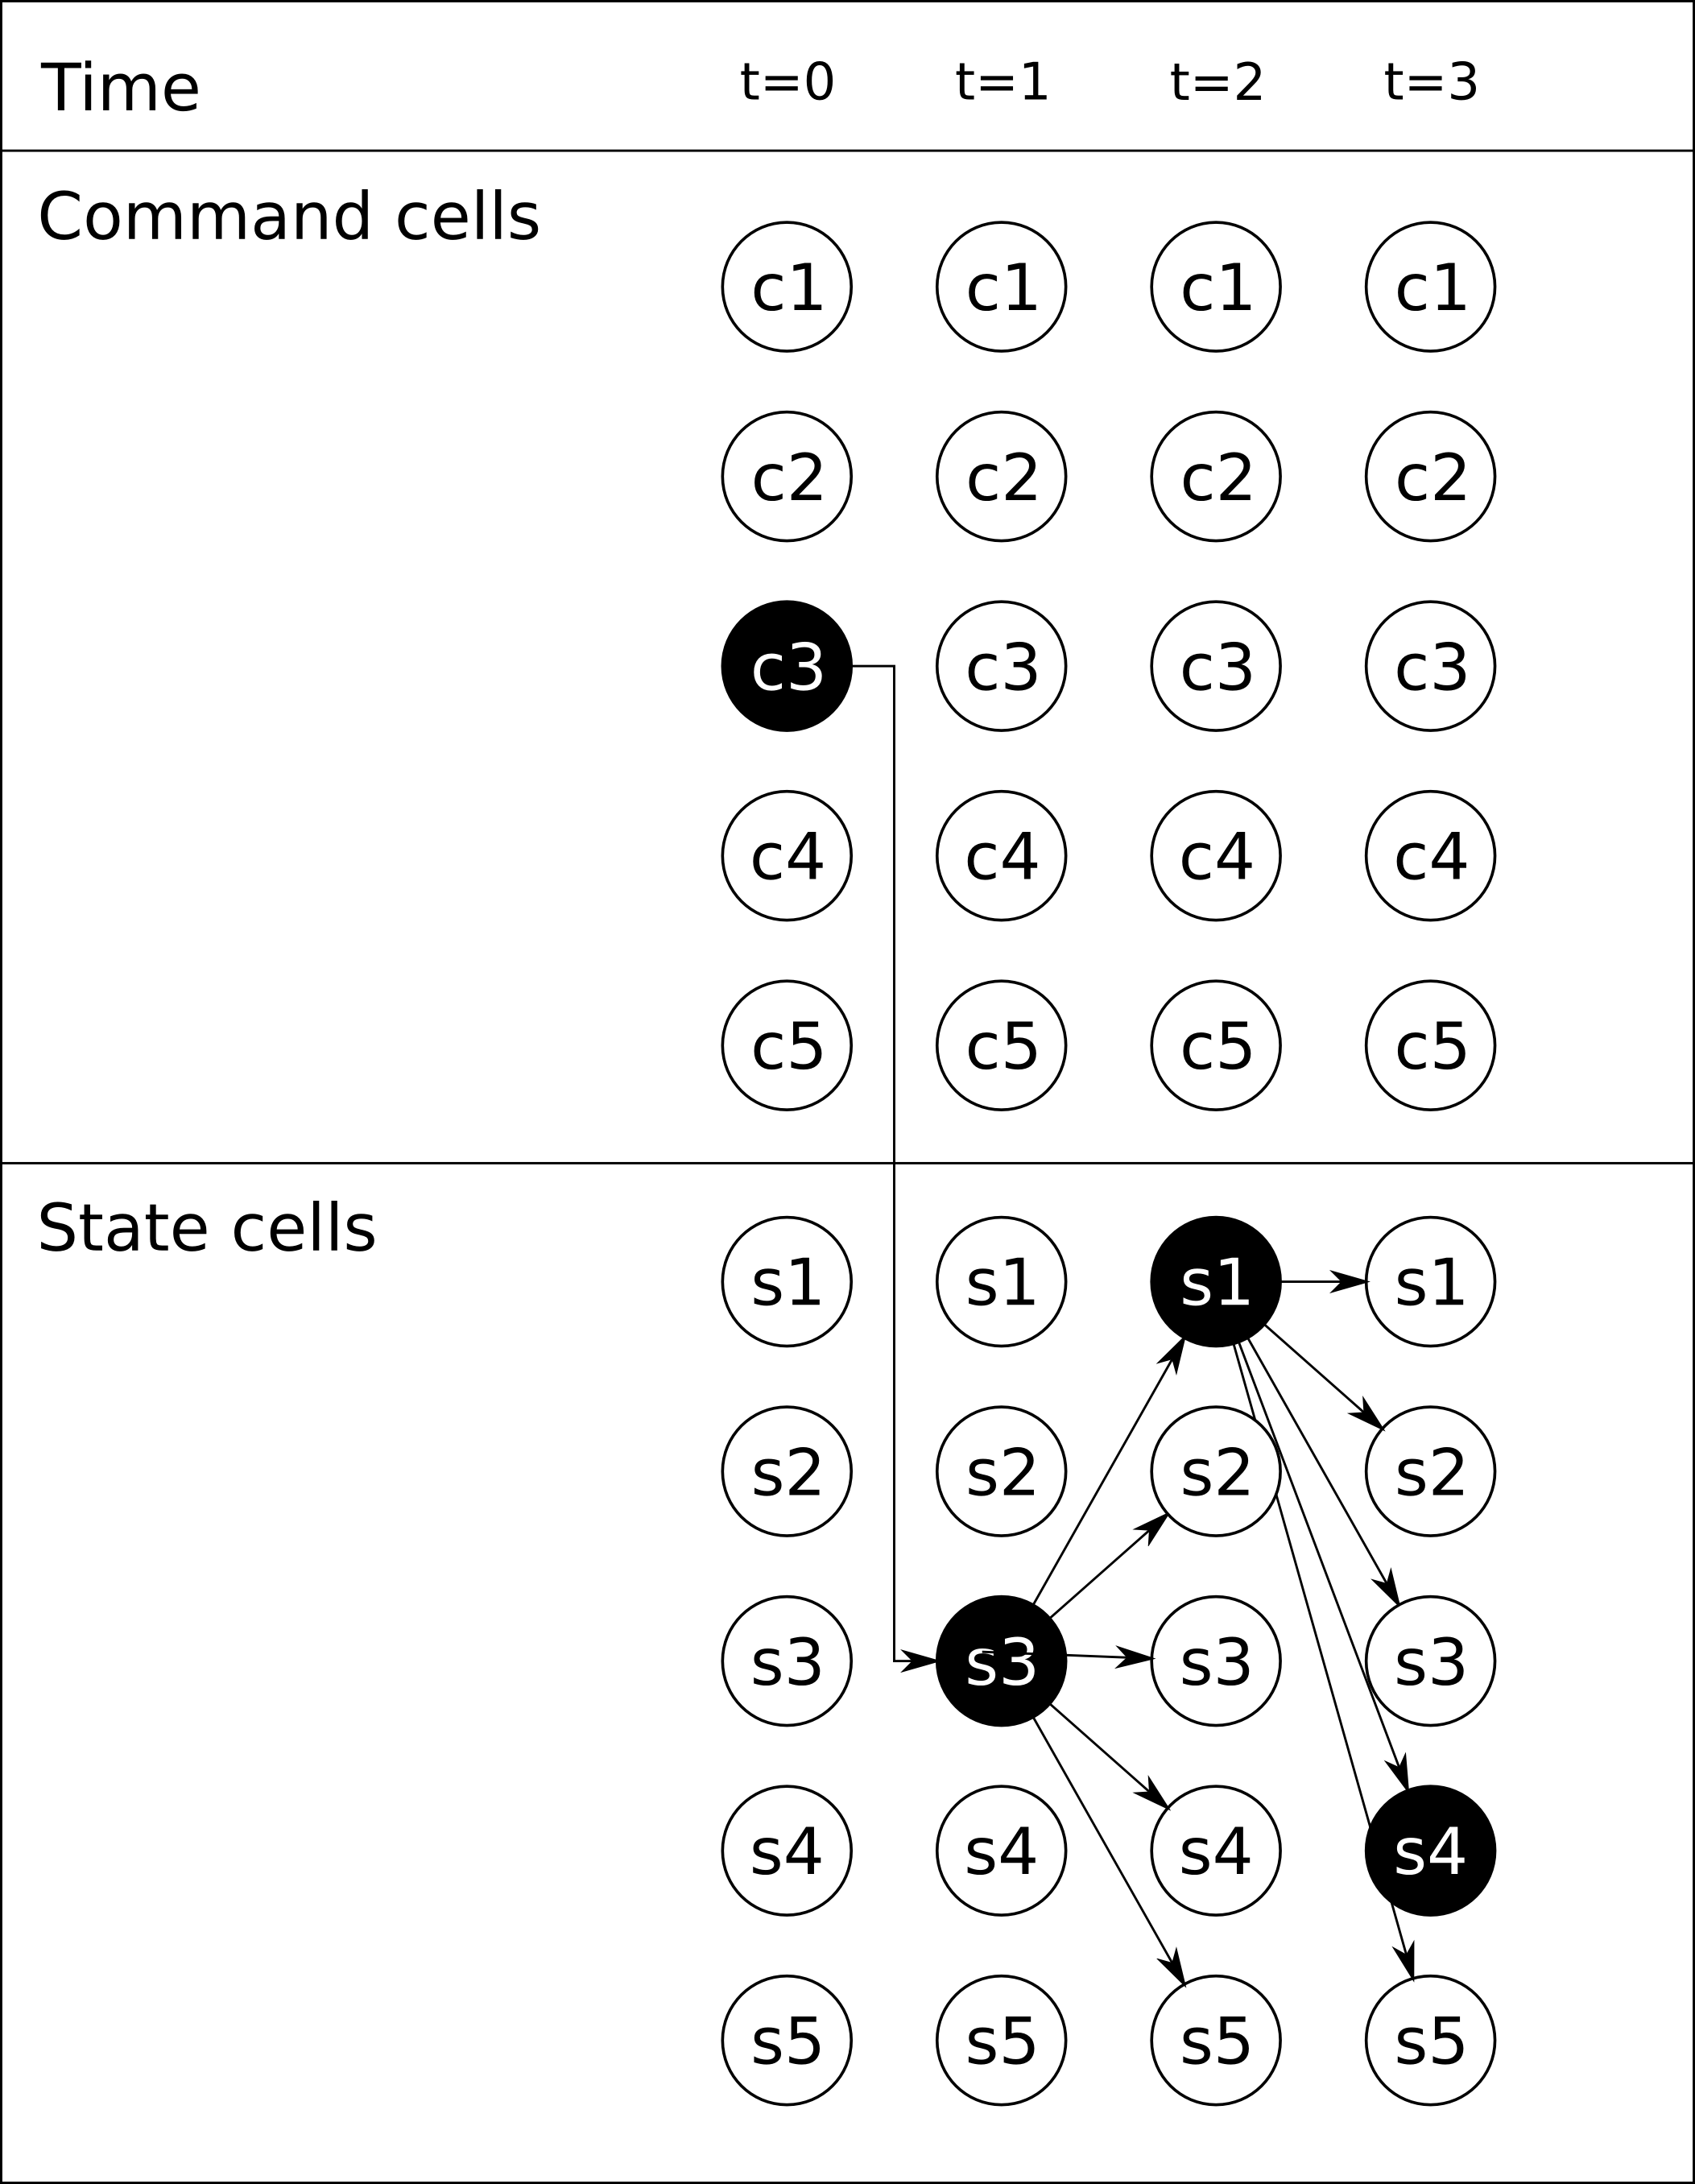
\includegraphics[width=\linewidth]{positive_model1.png}
\caption{Model 1. Each column represents a time step. Each row
  represents a particular neuron. Each circle represents a particular
  neuron at a particular time step; the circle is filled if that
  neuron fires at that time step. Arrows represent synapses between
  neurons, but most of them have been omitted for clarity. Note that
  each command cell $c_i$ excites the corresponding state cell $s_i$,
  and that each state cell $s_i$ can excite any other state cell.}
\label{fig-model1}
\end{figure}

\footnote{Justify microzone assumption}

This model (depicted in Figure \ref{fig-model1}) is the same as the
above, except that we don't assume that the states are linearly
ordered, and allow any state cell to influence any other state
cell. (We are only modeling cells within a single microzone, so really
we are only allowing state cells to influence related state cells.) At
every time step, if a command cell fired at the last time step, we
activate the corresponding state cell at this time step. If no command
cell fired at the last time step, we pick a state cell to make active
based on which state cell was active at the previous time step, and
the transition probabilities. If $s_i$ was active at the previous time
step, we pick $s_j$ with probability $p_{ij}$. Here $\sum_j p_{ij}=1$,
so the $p_{ij}$ (called the ``transition probabilities'') give a
probability distribution over $j$ for each fixed $i$; this is the
distribution of which $s_j(t)$ is one given the fact that
$s_i(t-1)=1$. The transition probabilities are learned, using a method
we will describe below.

This model is a slight modification of the Hidden Markov Model in
machine learning. The word ``hidden'' is slightly inaccurate for our
case, since we can observe the states via seeing which state cell
fires, and the data we are learning from includes the activity of the
command cells, which are in one-to-one correspondence with the state
cells. Also, we allow multiple outputs to be active at a given time,
while the standard HMM formulation has a single output at each time
step.

This model is able to learn sequences of outputs, and also to merge
together two actions that it already knows. The merging happens by
learning a transition between the state at the end of one action and
the state at the beginning of the next action. The model is not able
to learn waypoint transitions, as it does not have input from context
cells. All transitions must either be timed, or take place because of
input from command cells.

The system follows the following rules:
\begin{align*}
P \left[ s_i(t)=1 | c_i(t-1)=1 \right] &= 1 \\
P \left[ s_i(t)=1 | c_i(t-1)=0, s_j(t-1)=1 \right] &= p_{ji} \\
P \left[ o_j(t)=1 | t_j(t-1)=1 \right] &= 1 \\
P \left[ o_j(t)=1 | t_j(t-1)=0, s_i(t-1)=1 \right] &= q_{ij}, \\
\end{align*}
where the transition probabilities $p_{ji}$ and output probabilities
$q_{ij}$ are learned over time.

How do we learn the $p_{ij}$? Given a set of observations $s_1, \dots,
s_n$ over time, it is simply the observed conditional probability that
$s_{i}$ fired immediately before $s_j$, given the firing of $s_i$.
$$p_{ij} = \frac{\mbox{\# $t$ such that $s_j(t)=1, s_i(t-1)=1$}}
{\mbox{\# $t$ such that $s_i(t-1)=1$}}.$$

How do we learn the $q_{ij}$? Given a set of observations of $s_1,
\dots, s_n$ and $o_1, \dots, o_m$ over time, it is simply the observed
probability that $s_i$ fired immediately before $o_j$.
$$q_{ij} = \frac{\mbox{\# $t$ such that $o_j(t)=1, s_i(t-1)=1$}}
{\mbox{\# $t$ such that $s_i(t-1)=1$}}.$$

This model is not biologically feasible because there is no way to
ensure that only one state cell is active at a given time.

\subsection{Model 2: Hidden Markov Model with Context}

This model is the same as above, except that our transition
probabilities and output probabilities change based on context from
the context mossy fibers. Let the context mossy fibers be denoted by
$m_1, \dots, m_\ell$. We still only allow one state cell to be active
at a given time. We allow at most one command cell to be active at a
given time. We allow any number of context cells to be active at a
given time.

This model can be thought of as an average of multiple copies of the
previous model, one for each context mossy fiber that is active. This
allows us to learn waypoint transitions: if we have a context mossy
fiber that is active when the leg is in a certain position, then we
can learn to transition between the state we want to be in while
walking before the leg reaches that position, and the state we want to
be in after the leg reaches that position.

This model is the least biologically feasible, since there is no
mechanism to actually perform the averaging specified. We give it
solely for the intuition that the probability of a given state cell
triggering an output cell or another state cell can depend on the
activity of the context cells.

\footnote{What if no context mossy fibers are active? Would divide by zero}

The system follows the following rules:
\footnote{halfway through adding a null term}
\begin{align*}
P \left[ s_i(t)=1 | c_i(t-1)=1 \right] &= 1 \\
P \left[ s_i(t)=1 | c_i(t-1)=0, s_j(t-1)=1 \right] &= \frac{1}{1 + \# k : m_k(t-1)=1} \sum_{k : m_k(t-1)=1} p_{kji}  \\
P \left[ o_j(t)=1 | t_j(t-1)=1 \right] &= 1 \\
P \left[ o_j(t)=1 | t_j(t-1)=0, s_i(t-1)=1 \right] &= \frac{1}{1 + \# k : m_k(t-1)=1}
\sum_{k : m_k(t-1)=1} q_{kij},
\end{align*}
where the transition probabilities $p_{kji}$ and output probabilities $q_{kij}$ are learned over time.

How do we learn the $p_{kij}$? Given a set of observations of $s_1,
\dots, s_n$ and $m_1, \dots, m_\ell$ over time, it is simply the
observed conditional probability that $s_i$ fired immediately before
$s_j$, given the firing of $s_i$ and that the mossy fiber $m_k$ was
active at time $t-1$.
$$p_{kij} = \frac{\mbox{\# $t$ such that $s_j(t)=1, s_i(t-1)=1, m_k(t-1)=1$}}
{\mbox{\# $t$ such that $s_i(t-1)=1, m_k(t-1)=1$}}.$$

How do we learn the $q_{kij}$? Given a set of observations of $s_1,
\dots, s_n$, $m_1, \dots, m_\ell$, and $o_1, \dots, o_m$ over time, it
is simply the observed conditional probability that $s_i$ fired
immediately before $o_j$, given the firing of $s_i$ and that the mossy
fiber $m_k$ was active at time $t-1$.
$$q_{kij} = \frac{\mbox{\# $t$ such that $o_j(t)=1, s_i(t-1)=1, m_k(t-1)=1$}}
{\mbox{\# $t$ such that $s_i(t-1)=1, m_k(t-1)=1$}}.$$

\subsubsection{Sparsity in the Context Mossy Fibers}

This model works by essentially averaging together multiple copies of
the previous model, one for each mossy fiber that is active. It is
important to note that this version of the model cannot work well
unless each context mossy fiber is sparse, that is, fires rarely and
only in a narrow band of situations. If this is not the case, then we
will be averaging together models that are not specific to the
situation, and this will make it impossible for the transition
function to be appropriate - we will wind up transitioning to a random
state, essentially.

Fortunately, we have access to sparse context signals, since muscles
contain nerves that fire predominantly when the relevant muscle is a
particular length. 
\footnote{Look this up, I think they're called muscle spindles.}

\subsection{Model 3: Logistic Regression}

We now relax the restriction that only one state cell in a microzone
can be active at a particular time. The state of the system (not
counting inputs) is therefore represented by which subset of the state
cells are active at a given time step. This means that we have an
exponential number of states that the system can be in: if there are
$n$ state cells, then there are $2^n$ different possible combinations.

We maintain the one-to-one correspondence between the command cells
and the state cells, and we continue to assume that a state cell will
definitely fire when its corresponding command cell fired in the
previous time step.

In this model, we assume that each state cell makes a choice of
whether to fire at each time step. It makes this choice based on its
inputs: command cells, other state cells, and context cells. Let $s_i$
be a state cell. We assume that $s_i$ performs a relatively
straightforward computation: each of its inputs $u$ votes on whether
$s_i$ should fire, and it takes a weighted sum of these votes, and
makes its decision based on that. 

There are three kinds of deep nuclear cells. One projects to the
inferior olive, and can be ignored for now. The other two are
excitatory and inhibitory, respectively. We assume that all state
cells are excitatory, and that all inhibitory cells are output
cells. If this is true, a state cell can only increase the probability
that other cells fire, and thus an excitatory synapse from cell $s_1$
to cell $s_2$ can only be used to encode the information that $s_1$
firing should make $s_2$ more likely to fire at the next time step
(and the strength of the synapse can encode the strength of this
belief). If the reverse holds (i.e., if the event $s_1=1$ should be
taken as evidence that we shouldn't fire $s_2$), then the best the
synapse can do is to erode completely, so that $s_1$ does not excite
$s_2$ at all.

In the rest of this section, we give a formula for how a state cell
decides whether to fire, and then propose a learning rule that will
allow it to adapt the parameters of the formula correctly.

Let the state cells be denoted by $s_1, \dots, s_n$, the command cells
be denoted by $c_1, \dots, c_n$, the output cells be denoted by $o_1,
\dots, o_m$, and the context cells be denoted by $m_1, \dots, m_\ell$.

We will assume that the probability that $s_i(t)=1$ depends only on
the activity of $s_1(t-1), \dots, s_n(t-1)$, $c_i(t-1)$, and
$m_1(t-1), \dots, m_\ell(t-1)$. If $c_i(t-1)=1$, then we assume that
$s_i(t)=1$; that is, if the corresponding command cell fired at the
previous time step, then $s_i$ definitely fires at the current time
step. For the time being, let us assume that $c_i(t-1)=0$.

\begin{figure}
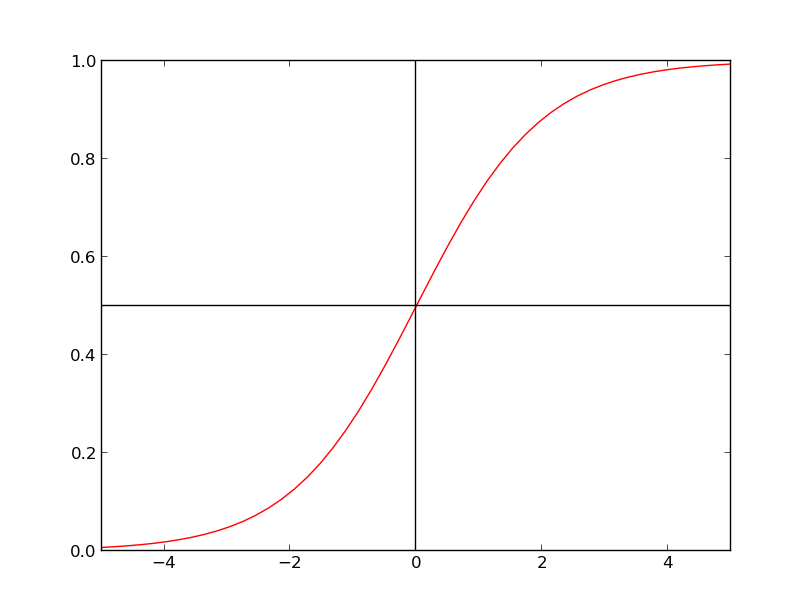
\includegraphics[width=0.5 \linewidth]{sigmoid.png}
\caption{The logistic sigmoid function $\sigma(x) = \frac{e^x}{1 +
    e^x}$}
\label{fig-sigmoid}
\end{figure}

We propose the following rule for $P[s_i(t)=1 | \{s_j(t-1)\}_j,
  \{m_k(t-1)\}_k]$, the probability that $s_i$ will fire at time $t$,
given the knowledge of which state cells and context cells fired at
time $t-1$:
\begin{align*}
P[s_i(t)=1 | \{s_j(t-1)\}_j, \{m_k(t-1)\}_k] &= \frac{e^{\theta_i +
    \sum_j w_{ij} s_j(t-1) + \sum_k x_{ik} m_k(t-1)} }{1 + e^{\theta_i +
    \sum_j w_{ij} s_j(t-1) + \sum_k x_{ik} m_k(t-1)}}.\\
\intertext{Letting $A_i(t) = \theta_i + \sum_j w_{ij} s_j(t-1) +
  \sum_k x_{ik} m_k(t-1)$,}
&= \frac{e^{A_i(t)}}{1 + e^{A_i(t)}}\\
&= \sigma\left(A_i(t)\right),\\
\end{align*}
where $\sigma(x) = \frac{e^x}{1 + e^x}$ is the logistic sigmoid
function (shown in Figure \ref{fig-sigmoid}).

It is worth pointing out that $w_{ij}$ will be fixed to zero whenever
there is no synapse from state cell $s_j$ to state cell $s_i$. When
there is no synapse from $s_j$ to $s_i$, $s_j$ does not get a vote on
whether $s_i$ should fire. It seems likely, however, that if $s_j$ is
a good predictor of $s_i$ at the next time step, the cerebellum will
likely grow the two neurons in such a way that they do form a synapse.

In order to have a neurologically realistic model, we need to have a
rule that can be applied locally by a single neuron in a small window
of time. Fortunately, this is relatively straightforward using
stochastic gradient descent.

Suppose that we observe the activity of the state cells, command
cells, and context cells over a period of time $t=0, \dots, T$. We
wish to set the parameters $\theta_i, w_{ij}, x_{ik}$ so that they
assign high probability to the sequence of firings that we actually
observed. This is done because we want future behavior of the state
cells to mimic the past behavior; this is one way to mathematically
express our desire that the cerebellum learn to predict its inputs and
then be able to repeat them semi-autonomously.

We assume that the probabilities at each state cell and each time step
are independent, so we can just multiply the probabilities:
\begin{align*}
P[\{s_i(t)\}_{i,t} | \{m_k(t)\}_{k,t}] &=
\prod_{i,t} P[s_i(t) | \{s_j(t-1)\}_j, \{m_k(t-1)\}_k]. \\
\intertext{This is more conveniently manipulated if we take the
  logarithm:}
\log P[\{s_i(t)\}_{i,t} | \{m_k(t)\}_{k,t}] &=
\sum_{i,t} \log P[s_i(t) | \{s_j(t-1)\}_j, \{m_k(t-1)\}_k]. \\
&= \sum_{i,t: s_i(t)=1} \log P[s_i(t)=1 | \{s_j(t-1)\}_j, \{m_k(t-1)\}_k] \\
& + \sum_{i,t: s_i(t)=0} \log P[s_i(t)=0 | \{s_j(t-1)\}_j, \{m_k(t-1)\}_k] \\
\end{align*}
Note that we are not conditioning on $c_i(t)$, because we wish to
learn the parameters that maximize the probability of observed
sequence of firings {\em without needing the commands to be
  issued}. This allows us to automate sequences of behavior that we
observe many times, allowing the cerebellum to take over the execution
of the behavior.

Now, we want to update the parameters $\theta_i, w_{ij}, x_{ik}$ to
increase this sum. This can be done via stochastic gradient ascent
(see the math chapter).

In our case, this yields:
\begin{align*}
\frac{\partial \log P[\{s_i(t)\}_{i,t} | \{m_k(t)\}_{k,t}]}{\partial w_{ij}}
&= \sum_{i,t: s_i(t)=1} \frac{\partial \log P[s_i(t)=1 | \{s_j(t-1)\}_j, \{m_k(t-1)\}_k]}{\partial w_{ij}} \\
& + \sum_{i,t: s_i(t)=0} \frac{\partial \log P[s_i(t)=0 | \{s_j(t-1)\}_j, \{m_k(t-1)\}_k]}{\partial w_{ij}} \\
&= \sum_{i,t: s_i(t)=1} \frac{\sigma'(A_i(t))}{\sigma(A_i(t))}
\cdot \frac{\partial A_i(t)}{\partial w_{ij}} + \sum_{i,t: s_i(t)=0}
\frac{(1-\sigma)'(A_i(t))}{1-\sigma(A_i(t))} \cdot \frac{\partial
  A_i(t)}{\partial w_{ij}}.\\
\intertext{Since $\sigma'(x) = \sigma(x)(1-\sigma(x))$, this simplifies to}
\frac{\partial \log P}{\partial w_{ij}}
&= \sum_{i,t: s_i(t)=1} (1 - \sigma(A_i(t))) s_j(t-1) + \sum_{i,t: s_i(t)=0}
-\sigma(A_i(t)) s_j(t-1).\\
\end{align*}
This can then be implemented locally (via stochastic gradient descent)
by the following update rule: 
\begin{align*}
\Delta w_{ij} &= \begin{cases} \eta (1-\sigma(A_i(t))) & s_i(t)=1, s_j(t-1)=1 \\
-\eta \sigma(A_i(t)) & s_i(t)=0, s_j(t-1)=1 \\
0 & s_j(t-1)=0\\
\end{cases}\\
&=  \begin{cases} \eta (1-P_{predicted}[s_i(t)=1]) & s_i(t)=1, s_j(t-1)=1 \\
-\eta P_{predicted}[s_i(t)=-1] & s_i(t)=0, s_j(t-1)=1 \\
0 & s_j(t-1)=0\\
\end{cases}
\end{align*}
This update rule is intuitively plausible:
\begin{itemize}
\item If $s_j(t-1)$ is zero, don't update $w_{ij}$, since $w_{ij}$ get
  multiplied by zero in $A_i(t)$, and thus $A_i(t)$ doesn't depend on
  $w_{ij}$.
\item If $s_j(t-1)$ is one and $s_i(t)$ is one, increase $w_{ij}$,
  since this observation suggests that $s_j(t-1)=1$ should be taken as
  evidence that $s_i(t)=1$. The strength of the update is proportional
  to $(1 - \sigma(A_i(t)))$; the lower our current estimate of the
  probability that $s_i(t)=1$, the more wrong we are, so the more we
  change the parameter $w_{ij}$.
\item If $s_j(t-1)$ is one and $s_i(t)$ is zero, decrease $w_{ij}$,
  since this observation suggests that $s_j(t-1)=1$ should be taken as
  evidence that $s_i(t)=0$. The strength of the update is proportional
  to $\sigma(A_i(t))$; the higher our current estimate of the
  probability that $s_i(t)=1$, the more wrong we are, so the more we
  change the parameter $w_{ij}$.
\end{itemize}

Based on similar calculations, we also have the following update rules
for other parameters:
\begin{align*}
\Delta x_{ik} &= \begin{cases} \eta (1-\sigma(A_i(t))) & s_i(t)=1, m_k(t-1)=1 \\
-\eta \sigma(A_i(t)) & s_i(t)=0, m_k(t-1)=1 \\
0 & m_k(t-1)=0\\
\end{cases}\\
\Delta \theta_i &= \begin{cases} \eta (1-\sigma(A_i(t))) & s_i(t)=1\\
-\eta \sigma(A_i(t)) & s_i(t)=0\\
\end{cases}\\
\end{align*}

The outputs are learned analogously. Let
$$B_i(t) = \varphi_i + \sum_{j} y_{ij} c_j(t-1) + \sum_j z_{ij} s_j(t-1) + \sum_j a_{ij} m_j(t-1).$$
Then
$$P[o_i(t) = 1 | \{c_j(t-1)\}_j, \{s_j(t-1)\}_j, \{m_j(t-1)\}_j]
= \sigma(B_i(t)),$$
and we get the following update rules
\begin{align*}
\Delta \varphi_i &= \begin{cases} \eta (1-\sigma(B_i(t))) & o_i(t)=1\\
-\eta \sigma(B_i(t)) & o_i(t)=0\\
\end{cases}\\
\Delta y_{ij} &= \begin{cases} \eta (1-\sigma(B_i(t))) & o_i(t)=1, c_j(t-1)=1 \\
-\eta \sigma(B_i(t)) & o_i(t)=0, c_j(t-1)=1 \\
0 & c_j(t-1)=0\\
\end{cases}\\
\Delta z_{ij} &= \begin{cases} \eta (1-\sigma(B_i(t))) & o_i(t)=1, s_j(t-1)=1 \\
- \eta \sigma(B_i(t)) & o_i(t)=0, s_j(t-1)=1\\
0 & s_j(t-1)=0\\
\end{cases}\\
\Delta a_{ij} &= \begin{cases} \eta (1-\sigma(B_i(t))) & o_i(t)=1, m_j(t-1)=1 \\
- \eta \sigma(B_i(t)) & o_i(t)=0, m_j(t-1)=1\\
0 & m_j(t-1)=0\\
\end{cases}
\end{align*}

\subsection{Comparison with Neurological Evidence}
\label{sec-mf-dcn-neuro}

\begin{pred}
These update rules are also sort of consistent with evidence from
studies of the mossy fiber collateral-deep nuclear cell synapse (see
Broussard). \footnote{\cite{pugh-raman, person-raman,
    zhang-linden}} Specifically, these studies found that long-term
potentiation of the synapse required the simultaneous activation of
the mossy fiber (so that the update is zero when $s_j(t-1)$ is zero,
as predicted) and hyperpolarization of the deep nuclear cell (which
corresponds to $\sigma(A_i)$ being low, and thus $(1-\sigma(A_i))$
being high, as predicted in the second case). Long-term depression of
the synapse required the simultaneous activation of the mossy fiber
and the depolarization of the deep nuclear cell (which corresponds to
$\sigma(A_i)$ being high, as predicted in the third case).

There are a few differences between the predictions of our model and
the existing evidence. The first difference is that we think LTP
should be restricted to cases where some ``ground truth'' signal fires
(a command cell firing for the case where the deep nuclear cell is a
state cell, an inferior olive cell firing for the case where the deep
nuclear cell is an output cell, or a pause in the firing of the
Purkinje cells, also for the case where the deep nuclear cell is an
output cell). For instance, the release of GABA from the Purkinje cell
could interfere with the LTP mechanism, so that its absence is
required for learning to take place. Similarly, we think that LTD
should be restricted to cases where the ground truth signal does {\em
  not} fire (or when the Purkinje cell {\em does} fire).

Finally, we think that LTP and LTD should occur in a linear fashion
compared to $1-\sigma(A_i)$ and $\sigma(A_i)$, respectively. Since
we're running it through some sort of nonlinearity like a sigmoid
function, the linearity is not the point - the point is that it should
be a continuous, monotonic function of the membrane potential, rather
than a step function. This is not an essential point, however; perhaps
the brain uses a step function to approximate the optimal rule, and it
still works.
\end{pred}

\subsection{Learned Reflexes}

Note that the context mossy fibers $m_1, \dots, m_\ell$ appear in the
output equations in the same form as the state cells do. This suggests
that the cerebellum can learn what we might call ``learned reflexes'':
an input from the spinal cord can enter the cerebellum and trigger
outputs with no involvement of the cerebral cortex. All that is
necessary for this to happen is that $m_k$ be a sufficiently good
predictor of $o_j$, and for there to be a synapse between from $m_k$
to $o_j$.

Similarly, if $m_k$ is a good predictor of $c_i$, then it is possible
to learn to trigger state cell $s_i$ directly from $m_k$.

\subsection{Learning AND's and OR's}

It is worth noting a few special cases that are in the space of
hypotheses that these algorithms are searching over. Firstly, as $a$
becomes larger, $\sigma(a\cdot x)$ grows closer and closer to the step
function 
$$f(x) = \begin{cases} 1 & x\ge 0\\
0 & x < 0\\ \end{cases}.$$
If we consider the case where
$$A_i(t) = a\cdot (-1.9 + 1 \cdot s_1 + 1\cdot s_2),$$ we see that
when $a$ is sufficiently large, $\sigma(A_i)$ approaches $1$ when
$s_1=s_2=1$ and $0$ otherwise. We can thus approximately represent an
AND function, which is $1$ when all of its inputs are $1$, and zero
otherwise. Since this is in our hypothesis space, we will learn
something close to it if that is the model that best explains the
data.

Similarly, using $$A_i(t) = a \cdot (-0.9 + 1 \cdot s_1 + 1 \cdot
s_2),$$ $\sigma(A_i)$ will approximately represent an OR function,
which is $1$ if any of its inputs are $1$, and $0$ otherwise.


\section{Psychophysical phenomena}

\subsection{The Darts Experiment}

\begin{figure}
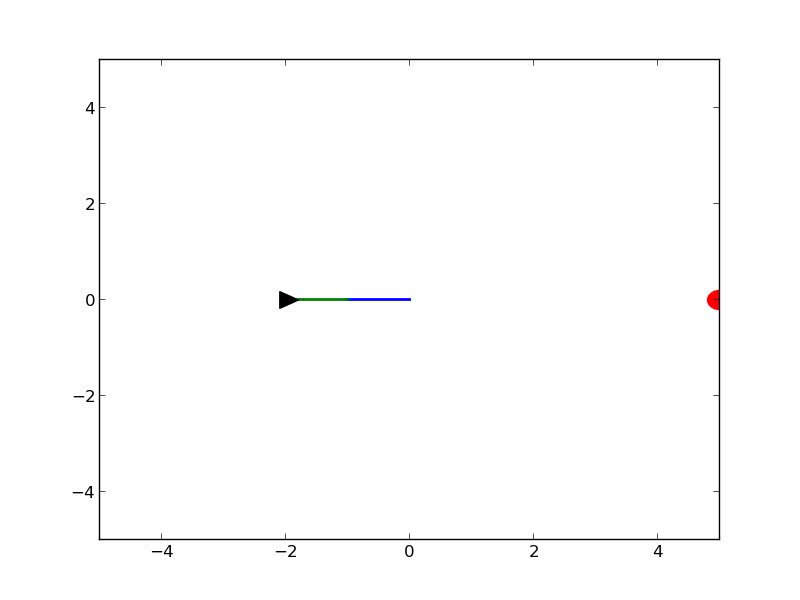
\includegraphics[width=0.5\linewidth]{darts-traj/frame1.png}
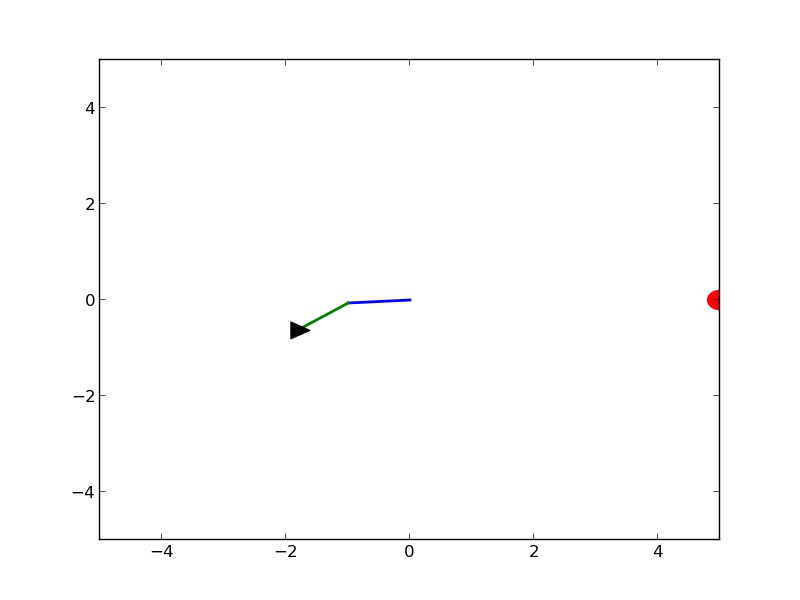
\includegraphics[width=0.5\linewidth]{darts-traj/frame2.png}
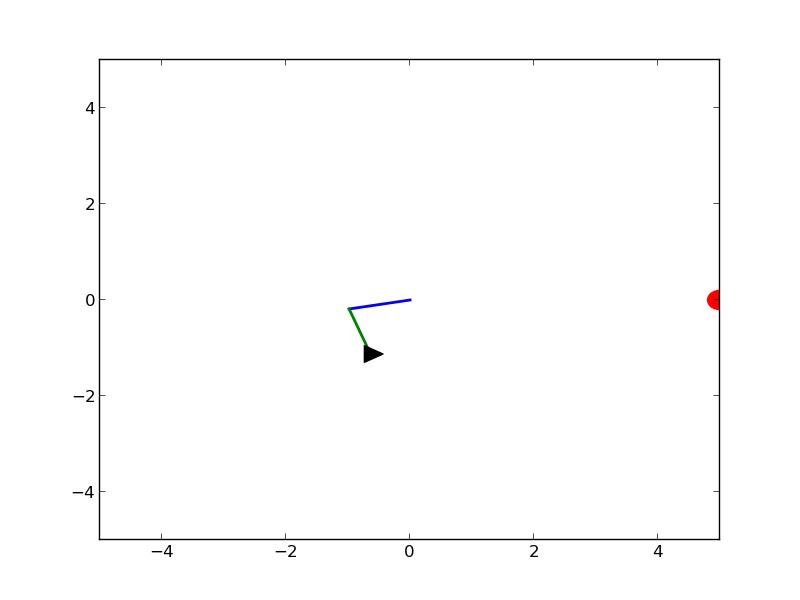
\includegraphics[width=0.5\linewidth]{darts-traj/frame3.png}
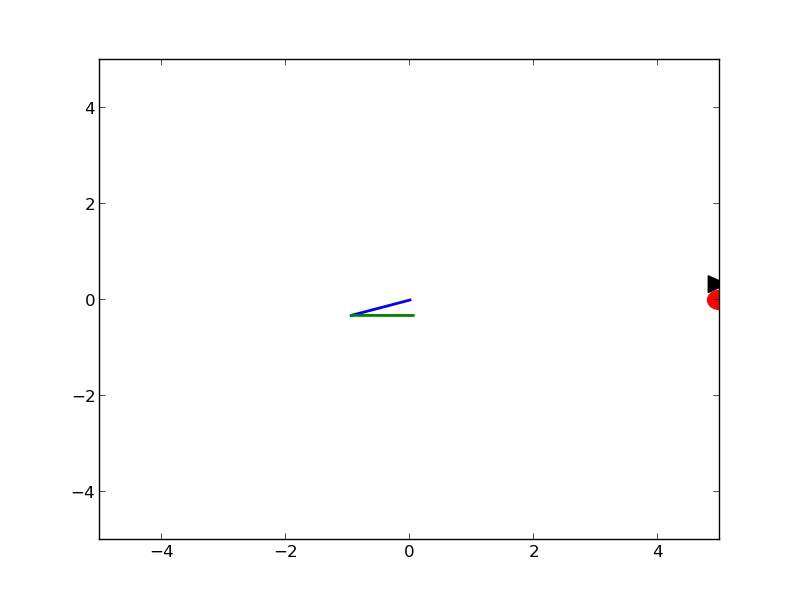
\includegraphics[width=0.5\linewidth]{darts-traj/frame4.png}
\caption{Time course of throwing a dart at a target. The arm has two
  articulation points, and it releases the dart when it thinks it will
  hit the target.}
\label{fig-darts1}
\end{figure}

\begin{figure}
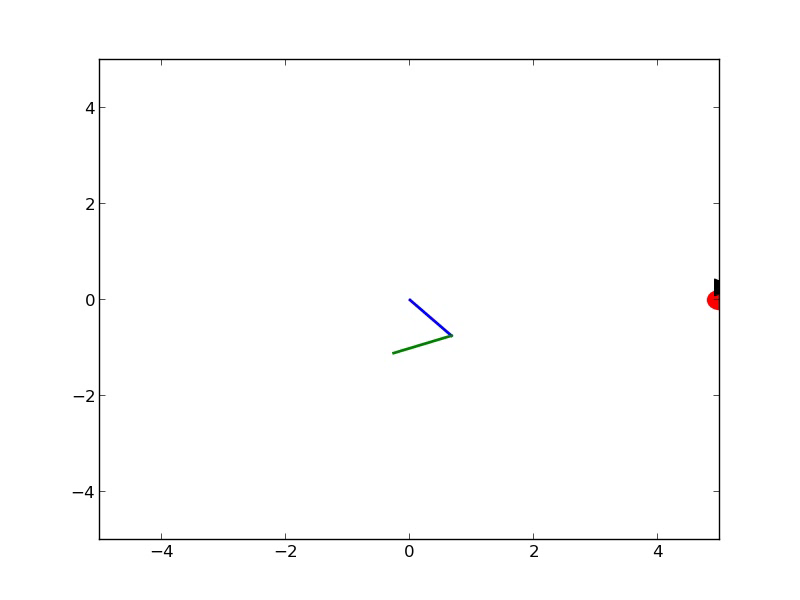
\includegraphics[width=0.5\linewidth]{darts-ex/1_normal_training.png}
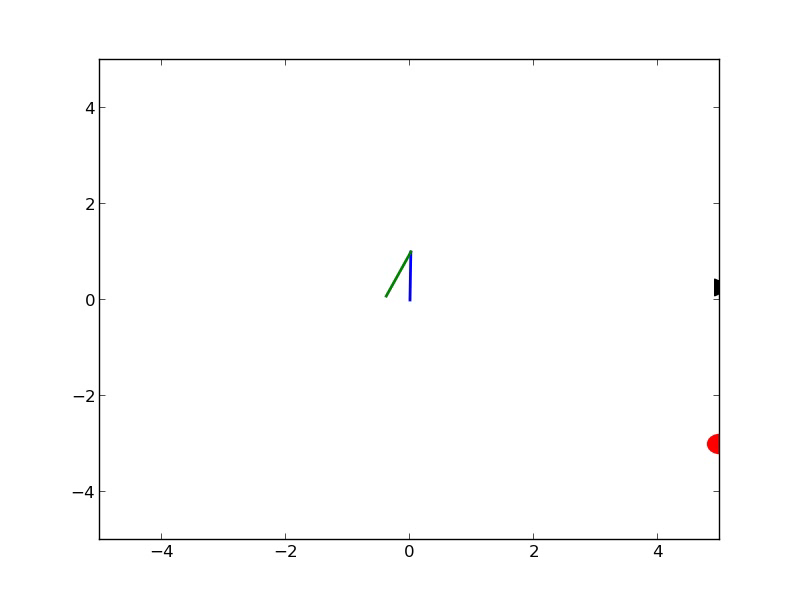
\includegraphics[width=0.5\linewidth]{darts-ex/3_prism_untrained.png}
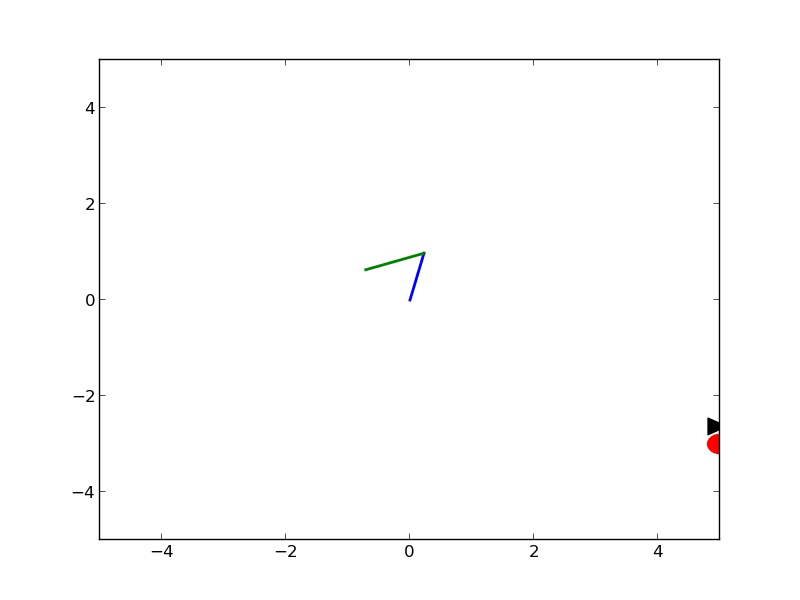
\includegraphics[width=0.5\linewidth]{darts-ex/4_prism_training.png}
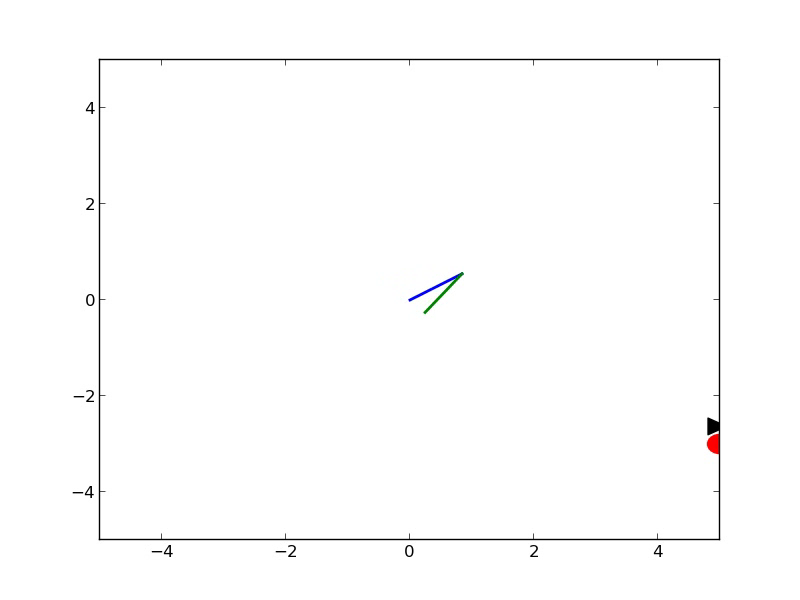
\includegraphics[width=0.5\linewidth]{darts-ex/5_prism_trained.png}
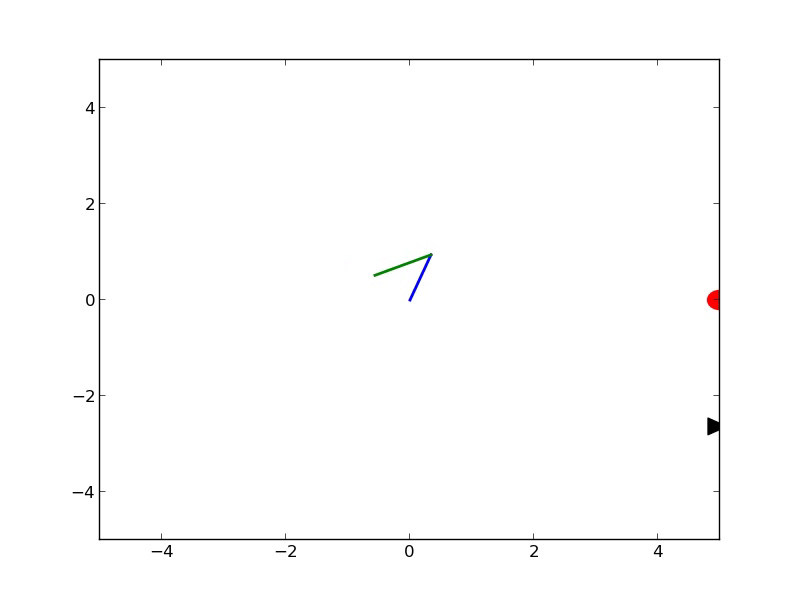
\includegraphics[width=0.5\linewidth]{darts-ex/7_normal2_untrained.png}
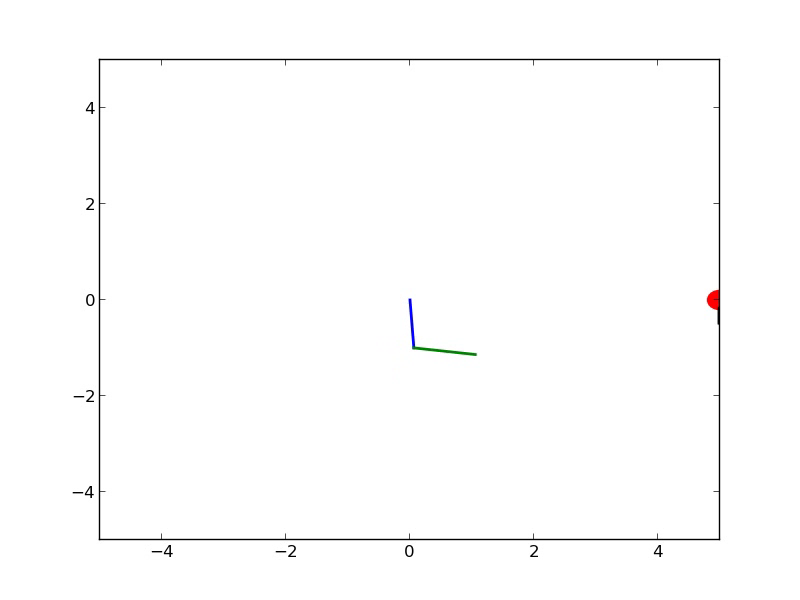
\includegraphics[width=0.5\linewidth]{darts-ex/8_normal2_training.png}
%%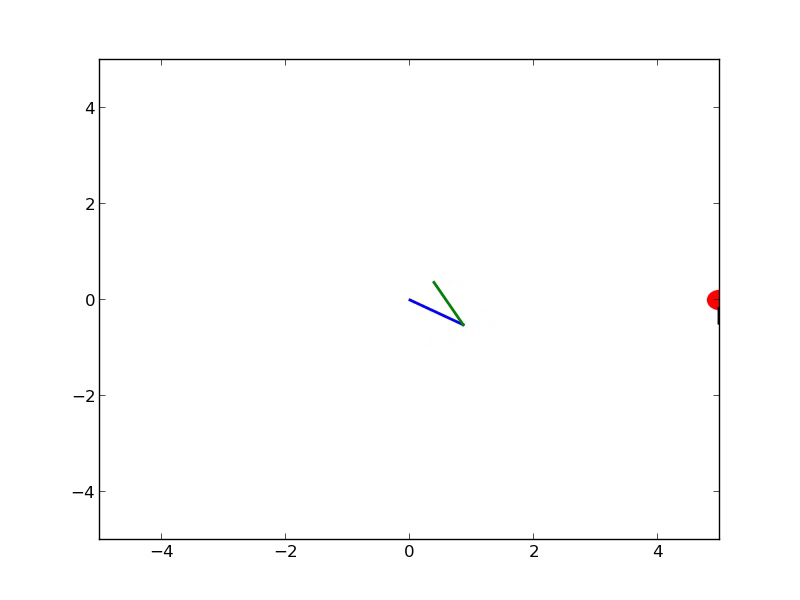
\includegraphics[width=0.5\linewidth]{darts-ex/9_normal2_trained.png}
\caption{Darts experiment. The red dot represents the target, and is
  translated to simulate the effect of prisms. In the first throw, the
  system is learning how to throw, and does so correctly after
  learning. In the second throw, it misses to the left because the
  target has moved. In the third throw, it learns to adapt to the new
  conditions. In the fourth throw, it has learned and uses a stored
  cerebellar program. In the fifth throw, when the original conditions
  have been restored, the system now misses to the right. In the sixth
  throw, the system has relearned the appropriate throwing technique,
  and again hits the target. (The dart has gone far in on the final
  throw, so it's hard to see, but it's close to the target.)}
\label{fig-darts2}
\end{figure}

In a classic experiment, Martin et. al. had subjects throw darts at a
target with and without prism glasses that distorted their view. The
prism glasses made it so that they had to look to the left to see
objects directly in front of them.

At the start of the experiment, the subjects threw darts normally, and
showed good accuracy: their throws were close to the target. The
subjects then donned the prism glasses. Their first throws were
displaced to the left, but gradually moved rightward as the subjects
adapted to the new setting. After they had fully adapted, they removed
the glasses. Their throws were then displaced to the right. While
making several more throws, their throws gradually moved leftward to
become accurate once again.

Our hypothesis is that
\begin{itemize}
\item The subjects had a cerebellar command (some combination of
  command cells firing, perhaps only one) that corresponded to
  throwing a dart at a target. This command depended for its accuracy
  on the situation that they were in front of the target and facing
  it.
\item After donning the prisms, the subjects continued to use the same
  cerebellar command, but since they were facing a different
  direction, the command resulted in a throw that was systematically
  skewed towards the left.
\item The subjects adapted to the novel conditions by sending the same
  cerebellar command in combination with another command that pulled
  the hand to the right as the throw was happening. The simplest
  hypothesis is that this other command was a non-cerebellar command,
  and that it resulted in the firing of the inferior olive cell
  associated with the action of moving the hand to the right.
\item The firing of the inferior olive cell led to the strengthening
  of the synapse between some state cell used in the course of the
  throwing action and the output cell corresponding to the rightward
  motion of the hand. This strengthening could take place either
  through the climbing fiber collaterals to the output cell, or via
  rebound excitation from a pause in the firing of the Purkinje cells
  that suppress the rightward motion (this pause in turn being caused
  by long-term depression triggered by the firing of the climbing
  fiber).
\item After adapting to the novel conditions, the cerebellar command
  for throwing a dart now incorporates the rightward motion of the
  hand, so that the command produces a throw systematically to the
  right of the direction the subject is facing.
\item After removing the prisms, the cerebellar command is still used,
  but it now produces a throw that is systematically to the right of
  the target. The subject adjusts by adding a command for leftward
  motion during the course of throwing the dart.
\item As before, the leftward motion triggers the inferior olive's
  climbing fiber and climbing fiber collaterals, causing the leftward
  motion to be added to the cerebellar command after a series of
  throws.
\item The subject now throws normally again. The leftward and
  rightward motions added to the cerebellar command counteract each
  other, and result in an accurate throw.
\end{itemize}

There is a slightly more complicated mechanism that would also explain
the data, which we term ``bleed-through''. The rightward motion could
be triggered by a cerebellar command, in which case the two cerebellar
commands would each be adapted with a little bit of the
other. Specifically, if two commands are issued in overlapping time
windows, each will observe the output of the other during their own
state transitions. This will result in an update of the state-output
cell synapse between the state cells of one action and the output
cells of the other action, as well as vice versa. It is also possible
that the transition synapses will be strengthened between the state
cells of one action and the state cells of the other action.

We implemented a simple model of the positive pathway to test that
this hypothesis would generate the observed data, and it does. We
created an arm with two joints (articulation points), which held a
dart at one end. It could then move the arm around the two joints to
generate movement, and release the dart when it will continue on to
hit near the target. The time course of throwing a dart is shown in
Figure \ref{fig-darts1}



\subsection{Dog scratch}

When you scratch a dog behind the ears, they will sometimes start to
move their leg in a way that looks like an abbreviated form of the
motion they would use to scratch their own ear. We believe that this
type of phenomenon is explained by the organization of the positive
pathway - basically, the context cells are relaying the information
that the ear is being scratched, which results in firing of the state
cells that code for this activity (remember that, in the logistic
regression model, the formulas look the same for state cell-state cell
synapses as they do for context cell-state cell synapses), which
results in the firing of output cells appropriate to scratching the
ear, which results in the observed motion.

\section{Questions}

\begin{q}
What is the topology of the state cells? That is, how do they connect
to one another, and how do they connect to other deep nuclear cells?
\end{q}


\section{Predictions}


\begin{pred}
\label{pred-positive-delay}
Learning at a state cell - output cell synapse should be maximized
when there is some delay between the firings. The delay should be on
the order of 100 msec, similar to the optimal delay for LTD in the
parallel fiber-Purkinje cell synapse. Recall that the inferior olive
cell's climbing fiber collateral triggers the output cell in order to
cause the firing of the output cell to coincide with whichever state
cell is currently active.

The delay is necessary, because the cerebrum is slower than the
cerebellum, and thus the signal from the inferior olive will always
arrive some interval after the ideal time for the output cell to have
fired. Maximizing learning with a delay would thus enable the
cerebellum to execute learned actions more quickly than the cerebrum
executed them during training.
\end{pred}

\begin{pred}
Without state cells, the cerebellum is only capable of learning and
executing an input/output mapping from command cells and context cells
to output cells. 

If the state cells were prevented from firing, the cerebellum would
still be able to maintain state by using the position of the body,
information which it can access as the output of the context mossy
fibers. Therefore, an animal with no state cells firing would probably
still be fairly coordinated, at least in the physical actions which
are the most easily observed cerebellar output.

Preventing the state cells and context cells from firing should
prevent the cerebellum from executing any learned sequential actions,
which should result in an animal whose movement is extremely
uncoordinated, resulting in movements similar to the movements of an
animal with extensive cerebellar damage. This should hold true even
though the cerebellum of the animal had previously learned many
activities.

If both state cells and context cells are prevented from firing, the
animal would still be able to use its cerebellum to map commands to
outputs, but there's no reason that this would be faster or more
responsive than a non-cerebellar pathway. Therefore, it seems unlikely
that the animal would regain its coordination if kept in this state.
\end{pred}

\begin{pred}
There should be pairs of cells in the deep cerebellar nuclei, one an
output cell and one a training suppression cell. They should have
similar firing patterns, and the training suppression cell should
project to the same inferior olive cell whose climbing fiber
collateral innervates the output cell.

The truth may be more complicated than this, but it should be the case
that each training suppression cell has a firing pattern that looks
like a nearby output cell, and that the inferior olive cell that
innervates the output cell has a similar firing pattern to the one
which the training suppression cell projects to.
\end{pred}


\end{document}
